\chapter{Dynamic Enrichment of Bayesian Small Sample, Sequential, Multiple Assignment Randomized Trial (snSMART) Design Using Natural History Data: A Case Study from Duchenne Muscular Dystrophy}
\label{chpt:snSMART}

\section{Introduction}
\label{s:intro}
\ac{DMD} is a potentially deadly inherited genetic disease with a birth prevalence of 19.8 per 100,000 live male births \citep{crisafulli2020global}. Patients often progressively lose the ability to walk or function independently and die at a young age from lung or heart problems. There is an unmet need for effective treatments in this patient population. Given the limited number of patients affected by \ac{DMD}, conducting separate dose-finding and randomized confirmatory trials is nearly impossible. Moreover, variability in disease progression, challenges in maintaining patient blindness to treatment, and ethical issues with long-term follow-up for placebo controls complicate trial design in \ac{DMD} and other rare diseases \citep{MUNTONI2022271}. This paper aims to address some of the challenges in \ac{DMD} and rare disease trial research and is motivated by the SPITFIRE trial (NCT03039686), a randomized, 2-phase, double-blind, placebo-controlled study (See Figure \ref{fig:SPITFIRE}) assessing the efficacy, safety, and tolerability of a new therapy (RO7239361) in 6-11 years old, ambulatory boys with \ac{DMD}.  We develop statistical methodology that improves the design and analysis of \ac{DMD} trials using all relevant information in the trial and external control data (i.e., relevant patient information gathered from sources outside of the prospective study).

In the SPITFIRE trial, patients were equally randomized to one of two doses (low and high) of treatment or a placebo arm in stage 1. After completion of stage 1 (48 weeks after the study entry), patients in the placebo arm were randomized to either high or low dose in stage 2. The trial's primary analysis planned to use only stage 1 data which ignores critical information generated in stage 2 about the drug. Moreover, the SPITFIRE design did not allow patients who performed poorly with low dose in stage 1 to receive high dose in stage 2. Finally, the SPITFIRE trial did not formally incorporate external control data. Further innovations are necessary to consider a trial design where patients receive multiple stages of treatment and analytic methods where treatment effect estimates consider data from all stages and from external controls.

This paper proposes a new \ac{snSMART} design with an efficient Bayesian analytic approach that synthesizes all relevant information and provides precise treatment effects for better decision-making about drugs in rare, life-threatening diseases like \ac{DMD}. However, combining data from different sources poses unique challenges, including the choice of relevant external information, potential conflict between external and concurrent control, and ``drift" in clinical outcomes between the two stages due to differences in the population. Lack of consideration of these factors may result in biased treatment effect estimates and increase false positive results. We modify existing \ac{snSMART} designs and develop a model-based approach that enables the use of external control data and combines data across trial stages resulting in more precise estimates of the treatment effects. Given the small sample size, the proposed model must be parsimonious and robust when there is conflict between different data sources. 

\section{SPITFIRE Trial: A Motivating Example of Phase IIb/III Trial in DMD}
\label{s:motivating}
We use the SPITFIRE trial setting and published results to demonstrate the utility of the proposed design and analytic approaches. Though SPITFIRE was stopped early for futility, it reflects the development paradigm for a new drug in many rare diseases. For example, a similar design was used for the ATMOSPHERE (NCT04704921) study. Note that, we have no intention to comment on or judge the clinical activity of the treatments involved or any decisions by sponsors or regulators associated with the trial or compound.

In the SPITFIRE trial, a total of 166 participants were randomized to receive one of two doses of RO7239361 or placebo (1:1:1) for 48 weeks at stage 1. After completion of stage 1, subjects entered an open-label stage where participants who originally received placebo were randomized into low or high dose groups, and all other participants stayed on their original treatment for up to 192 weeks. The primary and one of the secondary outcomes were the change (from baseline to week 48) of stage 1 \ac{NSAA} total score and \ac{6MWD} test.

The original SPITFIRE design is similar to an \ac{snSMART} \citep{tamura2016small} but lacks many fundamental features. SPITFIRE a) re-randomized only the participants in the control group in stage 2 and b) used only stage 1 data in the primary analysis. This differs from the \ac{snSMART} design used in the ARAMIS study (NCT02939573; as shown in Figure \ref{fig:standardsnSMART}; \cite{tamura2016small}), where data from both stages were used to estimate stage 1 treatment effects. There has been notable progress in \ac{snSMART} methods \citep{wei2018bayesian, wei2020sample, hartman2021design} that have been coded into an R package \citep{sidisnSMART}. Other \ac{snSMART} extensions include a group-sequential design that allows early stopping of an arm \citep{chao2020bayesian} and inclusion of multiple dose levels \citep{fang2021bayesian, fang2023comparing}.


\begin{figure}
\centerline{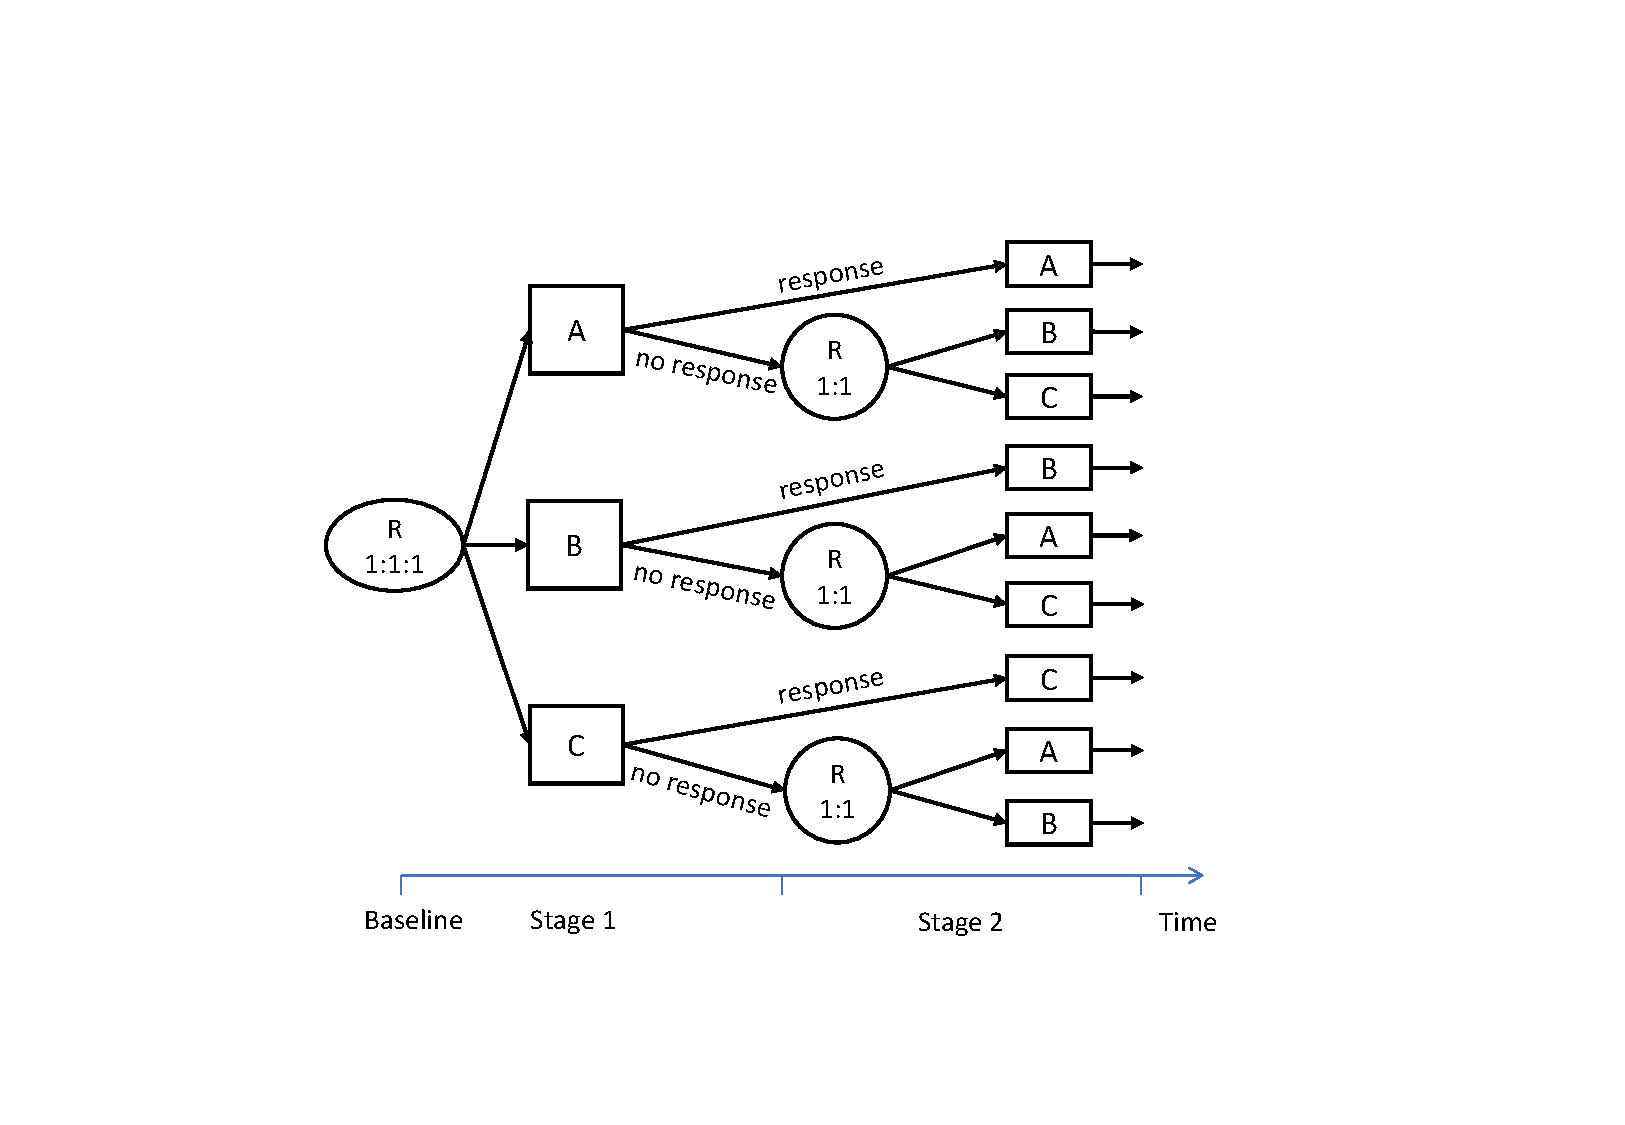
\includegraphics[width=12cm]{chapters/figures/standardsnSMART.pdf}}
\caption{Study design of a standard snSMART. In the study, participants are randomly assigned to one of three treatment options, referred to as arms A, B, and C, in a 1:1:1 ratio. They are then monitored for a specified period of time. Stage 1 responders will continue to receive the same treatment in stage 2, while the non-responders will be re-randomized to one of the other two treatment options in stage 2.}
\label{fig:standardsnSMART}
\end{figure}

In recent years, there has been an increased interest to consider the use of external control data to expedite the development of a new drug in rare diseases with an unmet medical need. Including external control data allows more patients to receive potentially more effective treatments than a placebo aiding in recruitment and retention, a smaller sample size, and therefore faster development. However, heterogeneity between external control and concurrent trial data is often a limiting factor in real-life applications. Yet, many approaches have been proposed to leverage external data in clinical trial while addressing heterogeneity between data sources, different types of available data (i.e., individual patient data or aggregated data), and outcomes of interest. Bayesian approaches for borrowing external control information differ in terms of assumptions regarding the relevance and exchangeability of external data with current trial data \citep{wadsworth2018extrapolation}. Use of the power prior approach directly down-weights the external control using fixed weights \citep{ibrahim2000power}. Dynamic methods adjust the informativeness of the prior based on measures of conflict between external control and the new trial data. Notable dynamic methods include normalized power prior \citep{duan2005modified, neuenschwander2009note}, commensurate priors \citep{hobbs2011hierarchical}, and robust meta-analytic-predictive priors \citep{spiegelhalter2004bayesian, neuenschwander2010summarizing, schmidli2014robust, neuenschwander2016use}. In the context of basket trials, \cite{ouma2022bayesian} explored Bayesian treatment effect borrowing and treatment response borrowing models that can be expanded to enable external control data borrowing. In addition to Bayesian methods, frequentist methods such as propensity score based matching \citep{rosenbaum1983central}, stratification, and inverse probability weighting \citep{lin2018propensity} are widely used when aggregate level information and baseline covariates are available. 

Existing \ac{snSMART} designs and methods do not incorporate external control data. In DMD, the \ac{DNHS} conducted by the \ac{CINRG}, which along with the PRO-DMD-01 Prospective Natural History Study (NCT01753804) and the University College London Natural History Study (NCT02780492) provide rich, external control information that can be combined with concurrent trial placebo data. Motivated by the \ac{DMD} setting, we aim to fill this gap with an innovative \ac{snSMART} design and Bayesian model as an alternative to the current practice of \ac{DMD} and rare disease drug development. The new approach proposes three key improvements to current \ac{snSMART} and rare disease design and methods: a) use of external control data to reduce the sample size of the placebo arm, b) allow stage 1 low dose nonresponders to receive higher dose in stage 2, similar to the design proposed by \cite{fang2021bayesian, fang2023comparing}, and c) use a Bayesian hierarchical model that dynamically incorporates external control data and borrows information across both trial stages. These features are extremely attractive in the rare disease setting where sample sizes and opportunities to perform clinical trials are limited. Our proposed design and methods assume a) the study condition remains relatively stable throughout the trial period (i.e., when there is no treatment effect, patients' primary outcomes do not fluctuate dramatically), b) an adequate washout period between the two trial stages, c) exchangeable treatment effects between stages, and d) similar external control and placebo effects. An \ac{snSMART} design is not appropriate for conditions that are not stable during the trial period, and we offer modifications to the model and sensitivity analyses to address other violations of these model assumptions.


\subsection{Proposed Modification for SPITFIRE Trial Design}

Our proposed \ac{snSMART} design is shown in Figure \ref{fig:codatasnSMART}, where eligible patients are randomized unequally (e.g., 1:2:2 or 1:3:3) between placebo, low dose, and high dose (e.g., of RO7239361) in stage 1. After 48 weeks, participants are re-assigned or re-randomized to either the same or a different dose of treatment depending on their initial treatment and post-baseline \ac{NSAA} total score. Here, we define a participant as a treatment responder at week 48 if their post-baseline \ac{NSAA} total score increases, stays the same, or does not decrease by more than 3.1 \citep{muntoni2018minimal}. Participants who received placebo in stage 1 are re-randomized with equal probability to either the low dose or high dose treatment arm in stage 2, regardless of their stage 1 response. This is beneficial to participants in the trial because everyone receives a dose of the treatment. This design differs slightly from the ones proposed by \cite{fang2021bayesian, fang2023comparing} in stage 2 for those who received low or high dose in stage 1. These slight modifications may make the design more patient-centered. Participants who received low dose in stage 1 are assigned to stay on low dose if they responded in stage 1 or switch to high dose if they did not respond. Participants who first received high dose and responded are re-randomized equally between low and high doses. However, the nonresponders to high dose are discontinued in stage 2. In most settings, the re-randomization of high dose responders is a viable design option because low dose may continue to be effective and possibly more tolerable. On the other hand, when the high dose proves ineffective for some participants, it is unlikely that a lower dose will yield better results for them. Additionally, administering an ineffective high dose that potentially poses higher toxicity is not ethical. Thus, we chose to exclude stage 1 high-dose nonresponders in stage 2.

\begin{figure}
\centering
\subfloat[]{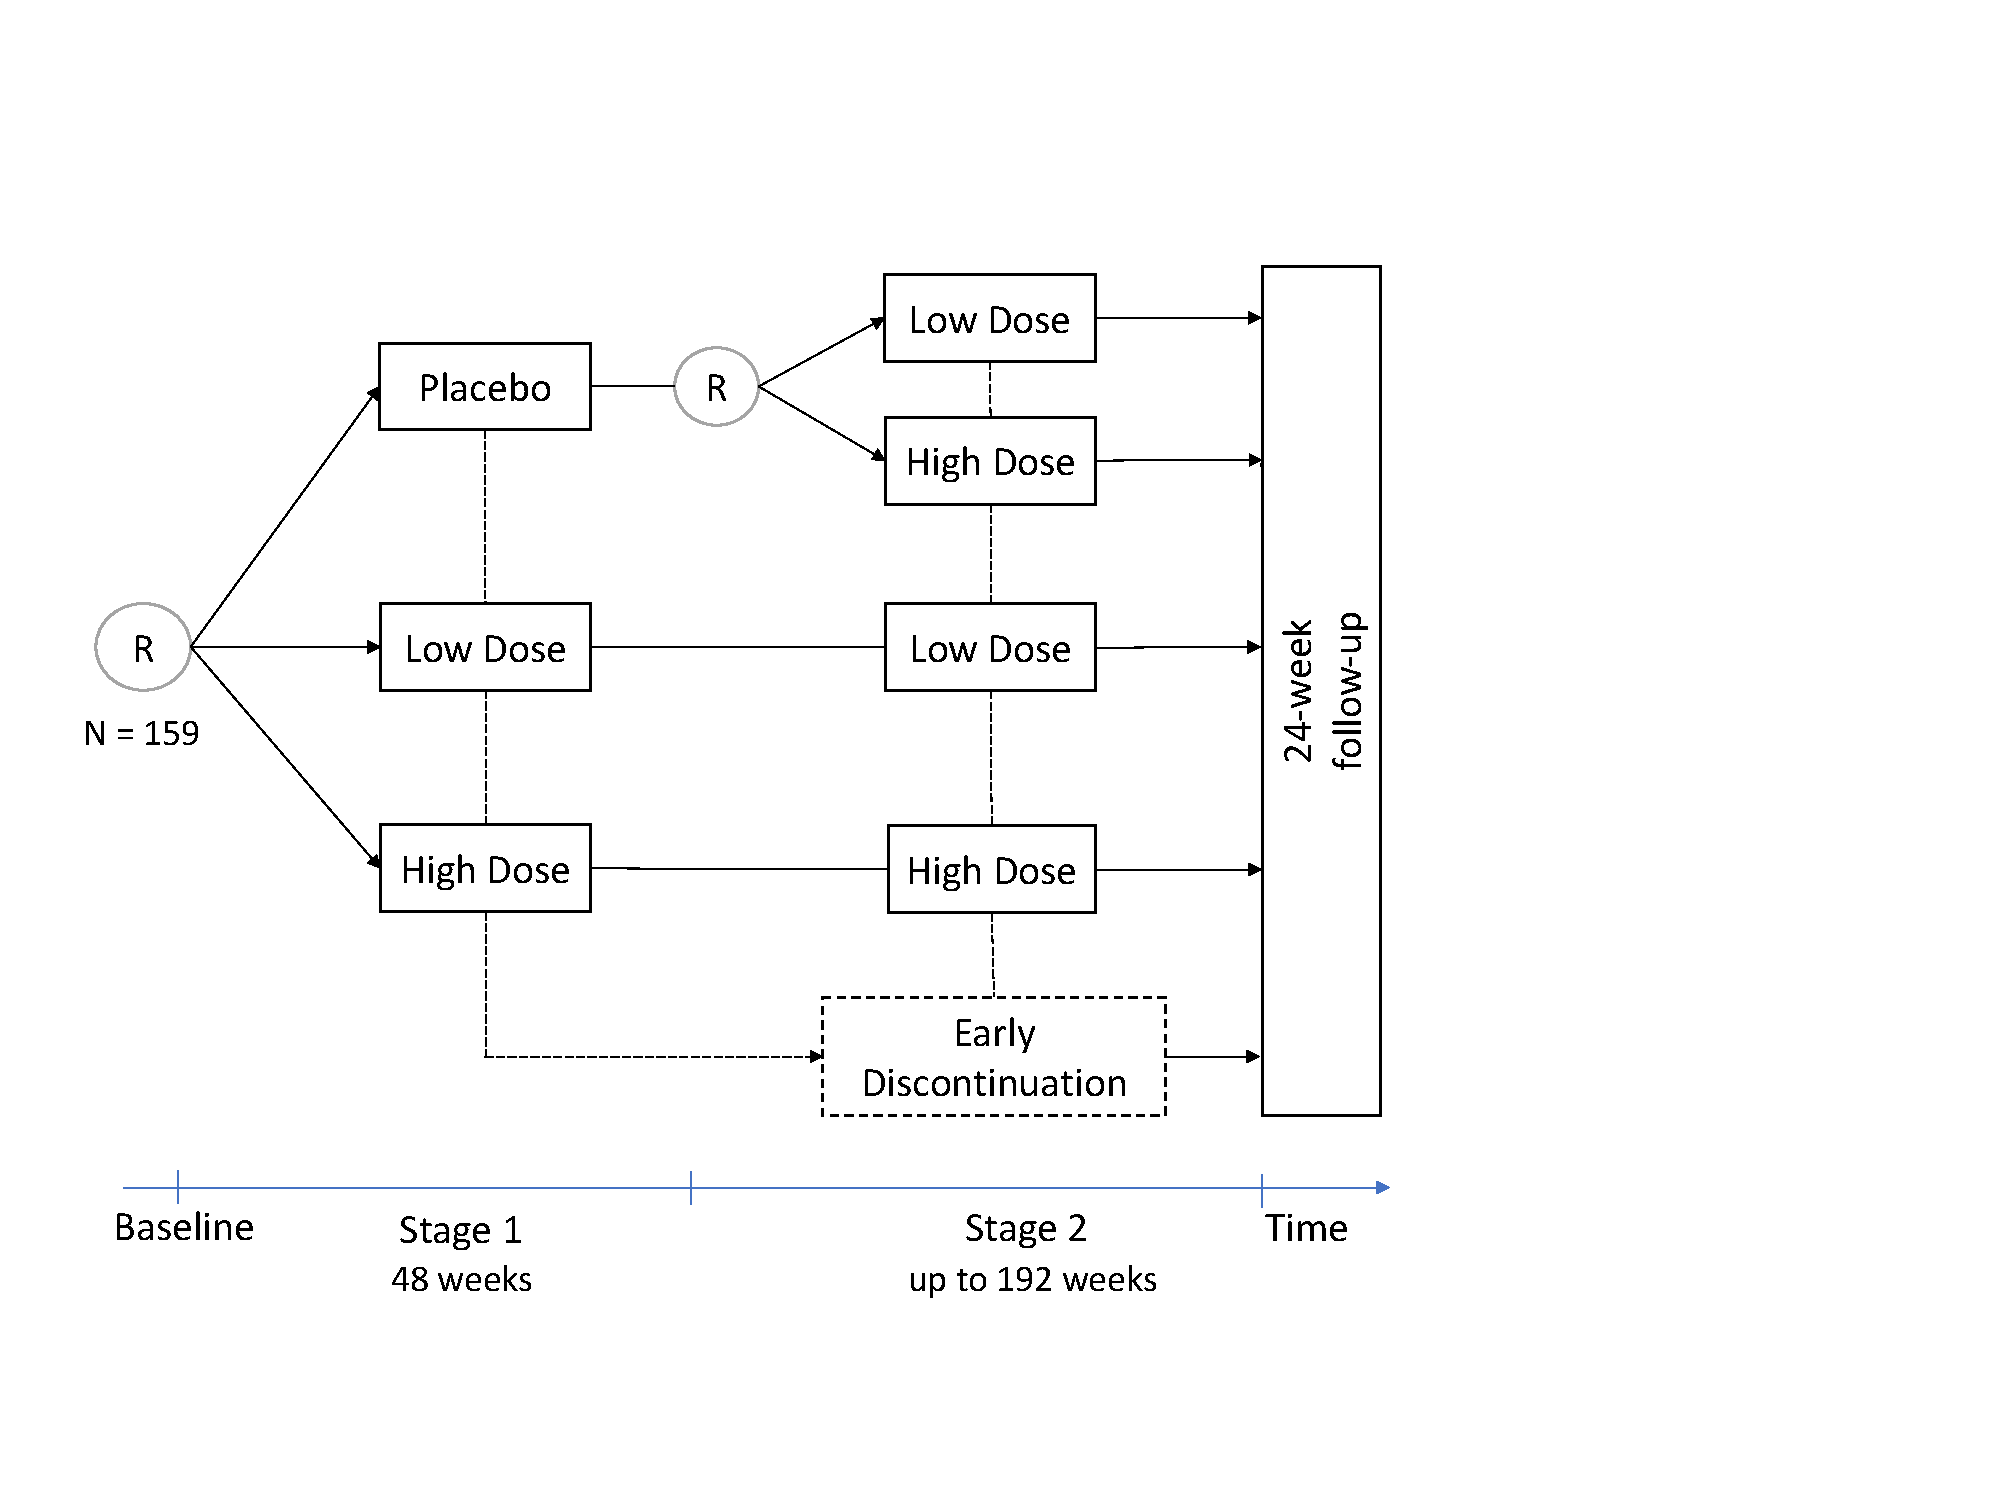
\includegraphics[width=10.7cm]{chapters/figures/Figure1.pdf}\label{fig:SPITFIRE}}
\\
\subfloat[]{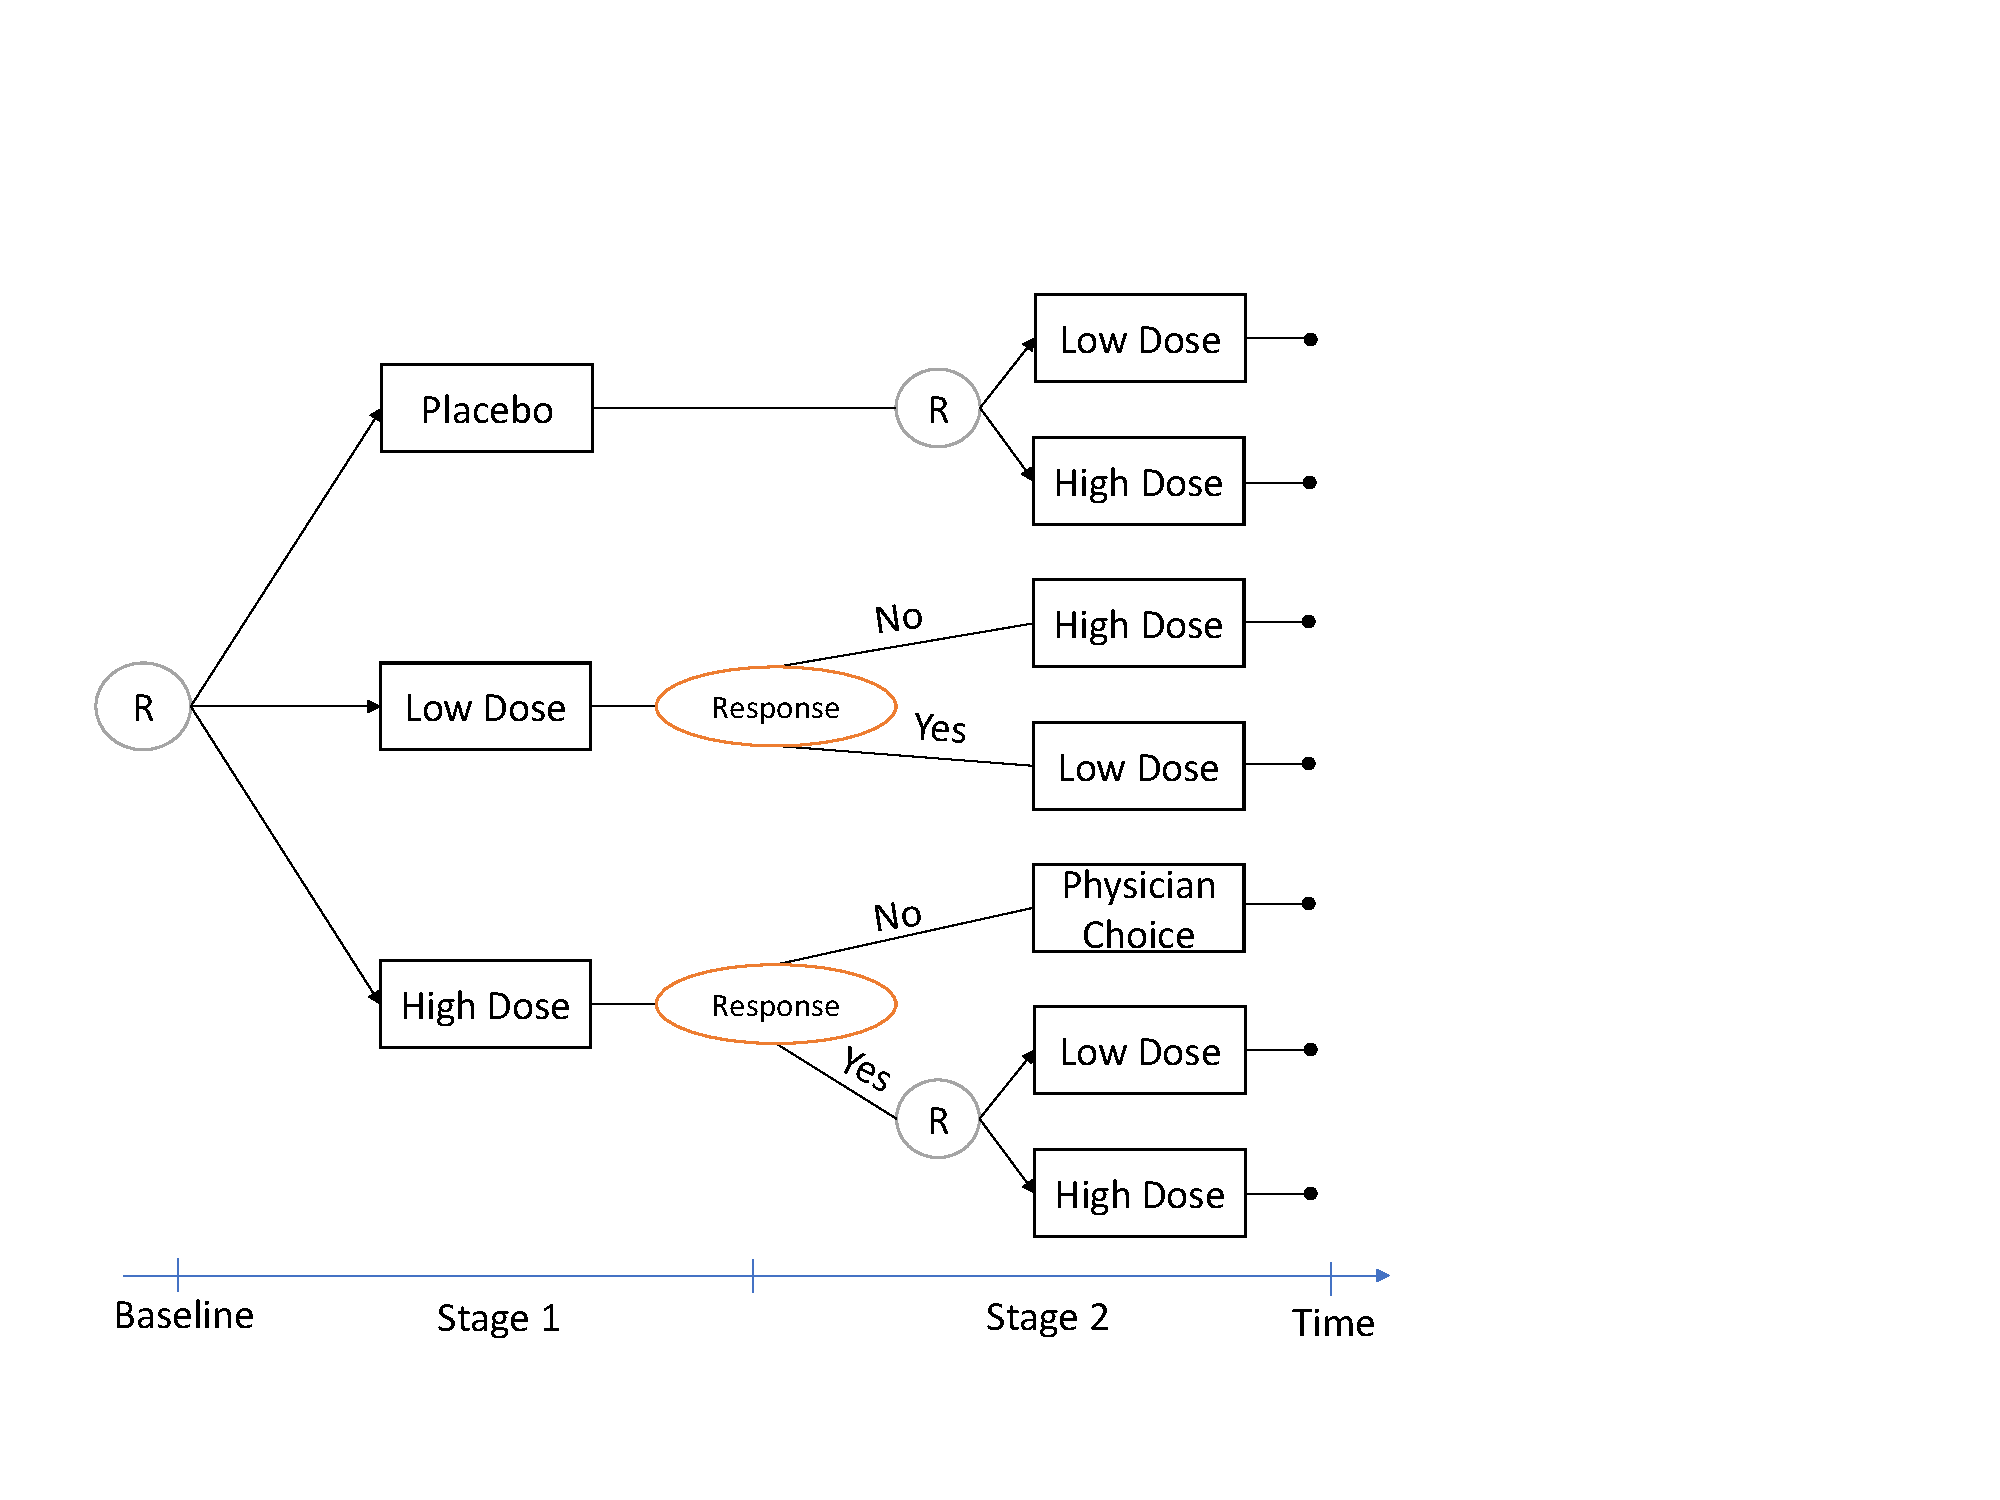
\includegraphics[width=10.7cm]{chapters/figures/Figure2.pdf}\label{fig:codatasnSMART}}
\caption{(a) Study design of the SPITFIRE trial (NCT03039686). (R) denotes randomization. (b) Study design of the proposed snSMART design that formally incorporates external control data. Participants are randomized (R) with 1:2:2 or 1:3:3 chances of receiving placebo, low dose, or high dose, respectively, in stage 1. At the end of stage 1, participants are assigned or re-randomized to their stage 2 treatment based on their stage 1 treatment and response status. Outcomes are collected at the end of stage 1 and 2.}
\end{figure}




\section{Methods} \label{s:methods}
 
The following notation is used in this section. $Y_{jk}$ and $\theta_{jk}$ denote the observed and underlying true mean change in outcome (e.g., \ac{NSAA} score) from the baseline values for stage $j = 1, 2$ and treatment $k = p$ (placebo), $l$ (low dose), $h$ (high dose), respectively. $Y_i'$ and $\theta_i'$ ($i = 1, 2, ..., n_c$) denote the observed and true placebo mean change in outcome from baseline for external control data. For example, in the SPITFIRE trial, $\theta_{1p}, \theta_{1l}$, and $\theta_{1h}$ represent the true mean change from baseline in the \ac{NSAA} total score or \ac{6MWD} for placebo, low, and high dose groups, respectively. The key estimands of interest are the stage 1 differences in effects between each dose and placebo ($\theta_{1l} - \theta_{1p}$,  $\theta_{1h} - \theta_{1p}$). Traditional analyses for $Y_{1k}$ (change from baseline in \ac{NSAA} or \ac{6MWD}) in SPITFIRE or similar studies include \ac{ANOVA}, \ac{ANCOVA}, or a conjugate Bayesian model (normal data and normal prior). Note that a traditional analytic method excludes external control data and uses only stage 1 outcomes. 

%The structure of the independent NNHM with external control data is very similar to that of the robust MAC-snSMART, except that under the independent NNHM, the stage 1 outcomes are assumed to be completely independent from the stage 2 outcomes in the new trial, which means that only stage 1 data is used to estimate the first stage treatment effects. Thus, formula \ref{eq:joint} is simplified to:
%\begin{equation}
%    Y_{ij}|\theta_{ij} \sim N(\theta_{ij}, s_{ij}^2); \quad i = 1, 2; \ j = p, l, h \\
%\end{equation}
%and formula \ref{eq:theta} is replace by:
%\begin{equation}\label{eq:ind}
%   \theta_{ij} \sim N(\mu_{ij}, \tau_{ij}^2); \quad i = 1, 2; j = l, h \\
%\end{equation}
  

%The \texttt{JAGS} code of all methods is provided in the Web Appendix ???.

\subsection{Bayesian joint stage model}
A modified version of the existing \ac{BJSM} by \cite{fang2023comparing} may be used to analyze our \ac{snSMART} design. Though it uses data from both stages, the existing \ac{BJSM} has not previously been presented to formally incorporate external data. One indirect or crude way to incorporate external control data is to use informative normal distribution priors for the model parameter associated with the placebo effect. For the \ac{BJSM}, normal distribution prior parameters may be derived using the method of moments approximation using external data, where the variance is further adjusted to ensure the desired prior effective sample size. 

Here, we use the summary-level \ac{DNHS} data to demonstrate the derivation of normal distribution prior parameters for BJSM:\\

\noindent Data source: Carefully matched \ac{DNHS} data as external controls.  \\
Mean test outcome change (from baseline to week 48):

\begin{center}
\begin{tabular}{ccc}
\hline
& NSAA Score & 6MWD \\
\hline
Mean & -1.04 & -22.36 \\
SD & 0.77 & 27.98 \\
\hline
\end{tabular}
\end{center}

\noindent Step 1: 

According to method of moments approximation, the normal priors for true placebo mean change in outcome ($\theta_{1p}$) should be $N(\mu = -1.04, sd = 0.77)$ under \ac{NSAA} Score, and $N(\mu = -22.36, sd = 27.98)$ under \ac{6MWD}.

\noindent Step 2: 

Decide on an \ac{ESS} we want to use. If \ac{ESS} $= E$, then the final normal priors for placebo should be $N(\mu = -1.04, sd = 0.77/\sqrt{E})$ under \ac{NSAA} Score, and $N(\mu = -22.36, sd = 27.98/\sqrt{E})$.
\subsection{Meta-analytic combined (MAC) approaches}

The meta-analytic combined, or MAC-snSMART, approach is a novel and unified analytic framework that incorporates ``all" relevant information for efficient estimation of stage 1 treatment effects, $\theta_{1p}, \theta_{1l}$, and $\theta_{1h}$. We use a Bayesian hierarchical model framework to dynamically borrow information from different sources (e.g., external control, stage 2). The framework consists of a series of models that link different sets of parameters (as shown in Figure \ref{fig:theta_diagram}). However, implementation of such a framework in the \ac{snSMART} setting requires innovation to a) handle heterogeneity between different sources of placebo data, b) account for the potential conflict between internal and external placebo data despite careful selection of external data, and c) account for selection bias due to non-randomized treatment assignments in stage 2 for participants who received low dose or did not respond to high dose in stage 1.

\begin{figure}
\centering
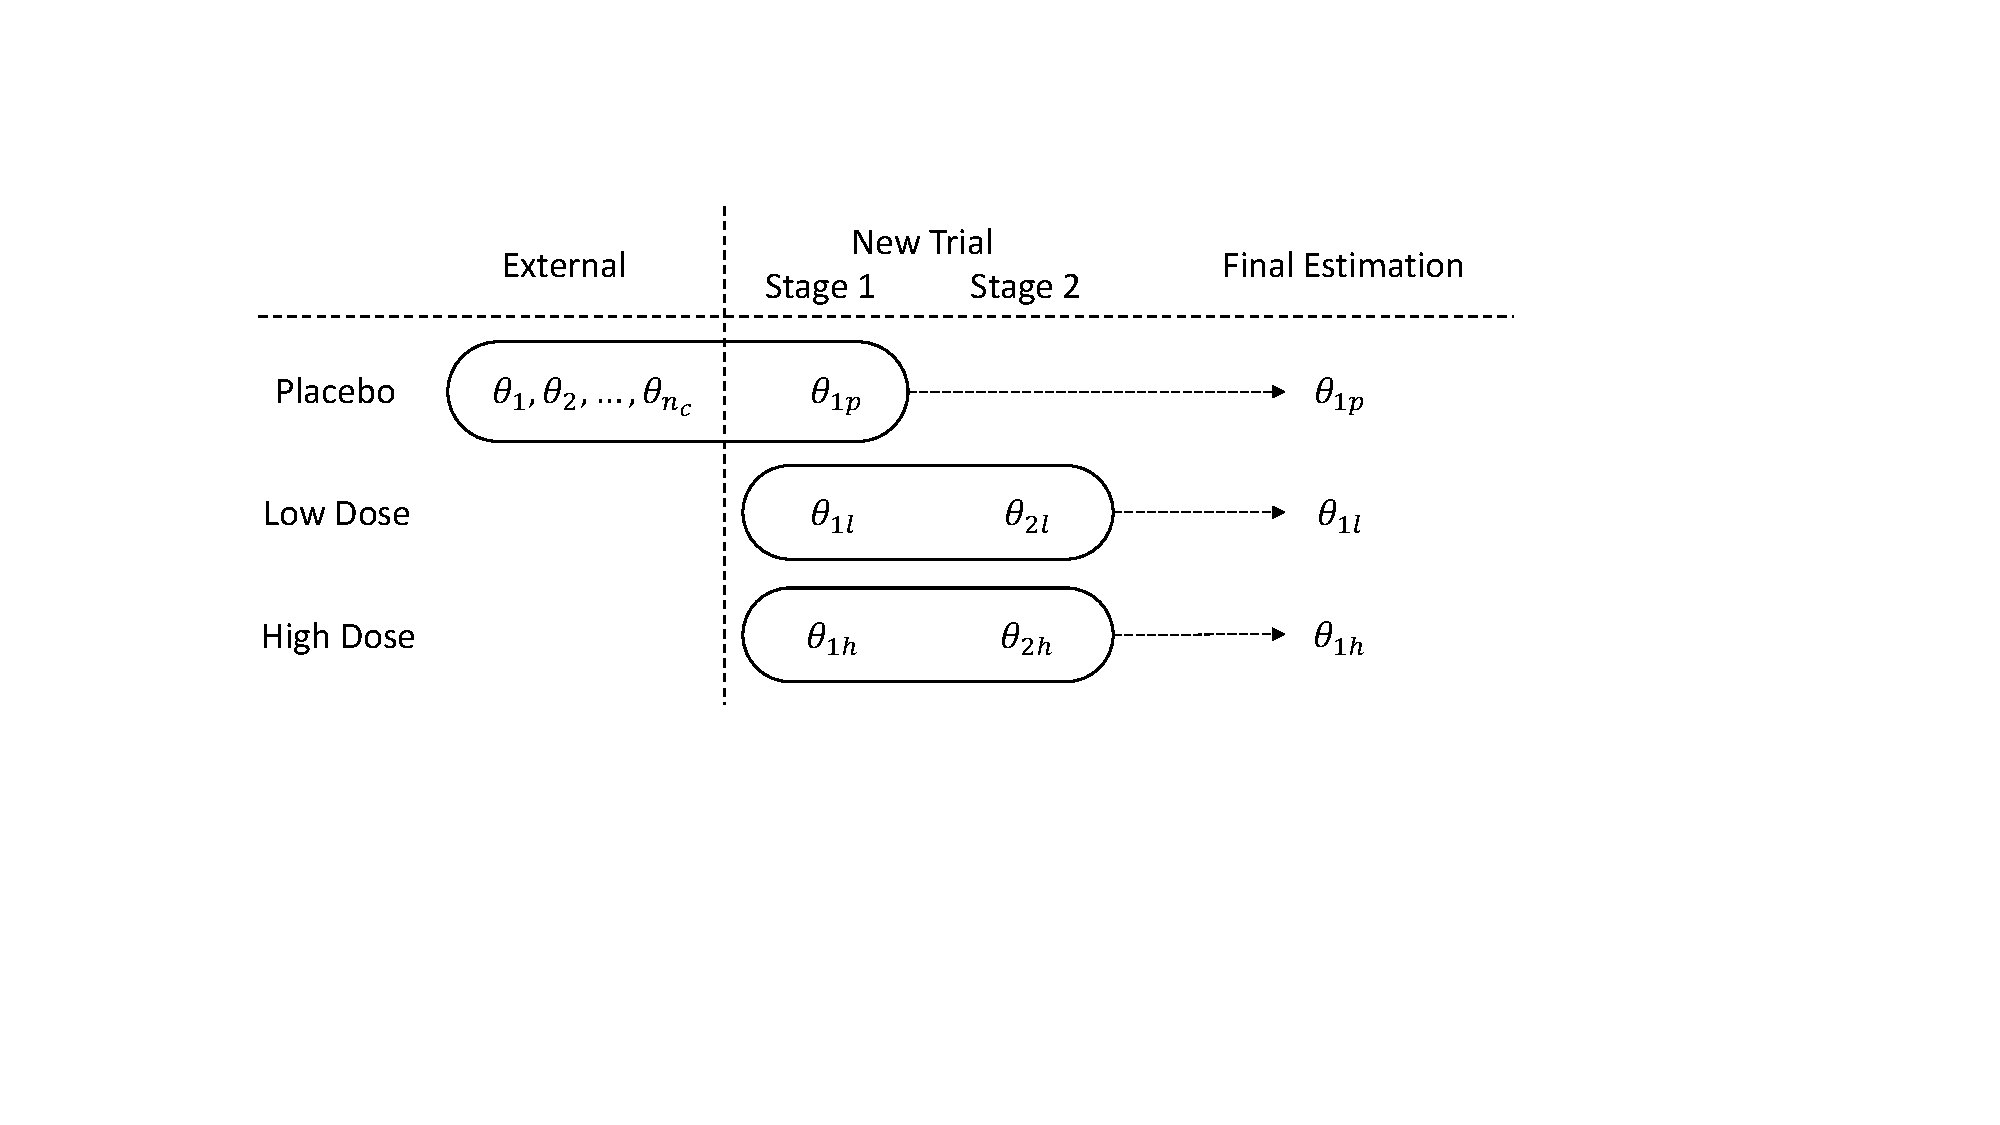
\includegraphics[width=14cm]{chapters/figures/theta_diagram.pdf}
\caption{Borrowing among treatment effects ($\theta$) in MAC-snSMART}
\label{fig:theta_diagram}
\end{figure}

\subsubsection{Use of external information for placebo} \label{sec:placebo}

Controlling for potential bias is a primary concern when considering external control data in a clinical trial. To handle bias due to potential unmeasured confounders in the design phase and increase the validity of results, statistical methods should be prespecified. To account for measured confounders, a first and critical step is careful selection of relevant external control data. \cite{pocock1976combination} and \cite{lim2018minimizing} proposed a set of criteria to assess the similarity between external and trial control data based on key aspects, including inclusion/exclusion criteria, endpoint definition, relevance of control treatment, distribution of demographic criteria, etc. Furthermore, matching techniques (e.g., propensity score matching) can be conducted to select external control patients used in the analysis to ensure appropriate balance of important prognostic factors. Irrespective of careful selection, the clinical outcome of interest may be variable across different sources due to associated intrinsic and extrinsic factors. A model-based approach is required to address these issues.  

For illustration we use summary level, external control data for this paper. However, the methodology is also applicable to patient-level data with important baseline covariates. Let, $Y_i'$ be the observed mean change from baseline for external placebo data source $i$. Furthermore, $Y_{i}'|\theta_{i}' \sim N(\theta_{i}', s_{i}'^2)$, where $i = 1, 2, ...n_c$, and $s_i'$ is known or derived from the $n_c$ external control data samples. Similarly, we assume $Y_{1p}|\theta_{1p} \sim N(\theta_{1p}, s_{1p}^2)$. For dynamic borrowing across different sources, we need a model that connects $\theta_i'$ and $\theta_{1p}$. A generic approach that connects $\theta_i'$ and $\theta_{1p}$ is a generalized hierarchical model which assumes exchangeability between internal and external control. This implies $\theta_{i}' |\mu_p, \tau_i' \sim N(\mu_p, \tau_i'^2)$ and $\theta_{1p}|\mu_p,\tau_{1p} \sim N(\mu_p, \tau_{1p}^2)$. If patient-level information about important predictors is available, the model can be extended via meta-regression. In contrast to the classical exchangeability assumption which assumes the same variance for $\theta_{i}'$ and $\theta_{1p}$, this structure accounts for external control data outliers by allowing for different between-trial standard deviations. However,  the exchangeability assumption results in overly optimistic borrowing and causes biased estimates when information from different sources conflicts. 

The amount of information borrowed from external control data while estimating the treatment effects for control, low, and high dose groups can be quantified. This amount of borrowed information can be expressed as the \ac{ESS}. Here, we use the expected local-information-ratio, which fulfills a basic predictive consistency requirement, as introduced by \cite{neuenschwander2020predictively}. We, like \cite{neuenschwander2020predictively}, recommend that the \ac{ESS} of each external control data set should not exceed the number of participants on the placebo arm in the trial. 

\subsubsection{Robustification} \label{sec:robust}
To avoid overly optimistic borrowing, we include a mixture model adopted from \cite{neuenschwander2016use} for $\theta_i'$ and $\theta_{1p}$.  The proposed model allows for non-exchangeability of any of the parameters associated with the placebo effect: 
\begin{eqnarray*}
\theta_i' \sim p_{i}*N(\mu_p, \tau_{i}'^2) + (1-p_{i})*N(m_i', v_i'^2) \\
\theta_{1p} \sim p_{1p}*N(\mu_p, \tau_{1p}^2) + (1-p_{1p})*N(m_{1p}, v_{1p}^2)
\end{eqnarray*}

$p_i$ and $p_{1p}$ are fixed a priori to reflect confidence about the similarity between external and concurrent control data. The values of $m_i', m_{1p}, v_i'$ and $v_{1p}$ are chosen based on expert knowledge. Weakly informative priors, such as priors worth approximately one observation \citep{kass1995reference}, are used for non-exchangeability parameters ($m_{i}'$, $m_{1p}$, $v_{i}'$, and $v_{1p}$). 

The mixture model introduced in here is a mixture of normal priors. For $\theta_{1p}$, we have $f(\theta_{1p}|p_{1p}, \mu_{p},\tau_{1p}, m_{1p}, v_{1p}) = p_{1p}N(\theta_{1p}|\mu_p,\tau_{1p}^2)+(1-p_{1p})N(\theta_{1p}|m_{1p},v_{1p}^2)$. Given that only summary-level treatment effect $Y_{1p}$ is used to conduct Bayesian inference, the likelihood function is the same as above. Here, we introduce the latent variable $Z_{1p}$, such that $P(Z_{1p} = 1) = p_{1p}$ and $P(Z_{1p} = 0) = 1-p_{1p}$, where $p_{1p}$ is the probability that $\theta_{1p}$ is fully exchangeable with external controls, and $1 - p_{1p}$ is the probability that $\theta_{1p}$ is non-exchangeable with external controls. The robustification component for stage 1 placebo arm can be expressed as $\theta_{1p}|(Z_{1p} = 1) \sim N(\mu_{p},\tau_{1p}^2)$ and $\theta_{1p}|(Z_{1p} = 0) \sim N(m_{1p}, v_{1p}^2)$.
Therefore, $Z_{1p}$ provides the label indicating the mixture components from which the observations have been generated. Now the posterior probability that $\theta_{1p}$ has been generated from $N(\mu_p, \tau_{1p}^2)$ is:
\begin{equation*}
    P(Z_{1p} = 1|\theta_{1p}, \mu_{p},\tau_{1p}, m_{1p}, v_{1p})=\frac{p_{1p}N(\mu_p, \tau_{1p}^2)}{p_{1p}N(\mu_p, \tau_{1p}^2)+(1-p_{1p})N(m_{1p}, v_{1p}^2)}.
\end{equation*}
Similarly, we could create latent variables $Z_i$ for $\theta_i$, where $i = 1, 2, ... n_c$, and use the same structure as above to obtain the posterior probability that $\theta_i'$ has been generated from $N(\mu_p, \tau_i'^2)$. 

Based on conjugate priors, the posterior distribution of $\theta_i'$ and $\theta_{1p}$ are mixtures of normal distributions. Specifically, for $\theta_{1p}$, when equation 1 is not considered, the posterior mean is:
\begin{equation*}
    p_{1p}(\eta_{1p}\hat{\mu}_p+(1-\eta_{1p})Y_{1p})+(1-p_{1p})\frac{m_{1p}(s_{1p}^2+\tau_{1p})+Y_{1p}v_{1p}^2}{s_{1p}^2+\tau_{1p}+v_{1p}^2}
\end{equation*}
where $\hat{\mu}_p = (\omega_{1p}Y_{1p} + \sum_{i}{\omega_{i}'Y_{i}'})/\omega_{sum}$ is the posterior mean of $\mu_p$, $\omega_i' = (s_i'^2+\tau_i'^2)^{-1}$ and $\omega_{1p} = (s_{1p}^2+\tau_{1p})^{-1}$ are inverse variance weights, $\omega_{sum}$ is the sum of all inverse variance, and $\eta_{1p}=s_{1p}^2/(s_{1p}^2+\tau_{1p})$. 

We refer to the method as ``robust MAC-snSMART" if the robustification component is included in addition to the structure outlined in Section \ref{sec:placebo}. If this component is not included ($p_{i}=p_{1p}=1$), the method is simply referred to as ``MAC-snSMART".

\subsubsection{Combining evidence for low and high dose groups}

According to the proposed \ac{snSMART} design, a participant may follow one of seven different treatment sequences: $(1p, 2l)$, $(1p, 2h)$, $(1l, 2l)$, $(1l, 2h)$, $(1h, 2l)$, $(1h, 2h)$, and $(1h,$ \emph{No stage 2 treatment}). 
For each of the first six groups, the joint distribution of outcomes from stages 1 and 2, $Y_{1k}$ and $Y_{2k'}$, follows:
\begin{equation}\label{eq:joint}
\begin{bmatrix} Y_{1k} \\ Y_{2k'} \end{bmatrix} \sim MVN\left(\\ \begin{bmatrix} \theta_{1k} + B \\ \theta_{2k'}\end{bmatrix}, \begin{bmatrix} s_{1k}^2 & s_{kk'}s_{1k}s_{2k'}\\ s_{kk'}s_{1k}s_{2k'} & s_{2k'}^2\end{bmatrix}\right),
\end{equation}   
where $k = p, l, h; \ k' = l, h$. $s_{jk}$ can be estimated based on observed data in the \ac{snSMART}. $s_{kk'}$ denotes the correlation between stage 1 treatment $k$ outcomes and stage 2 treatment $k'$ outcomes. Note, $B$ is a selection bias correction term. This selection bias is due to design since those who receive low dose in stage 1 are not re-randomized and those who do not respond to high dose in stage 1 are excluded in stage 2. Given that we know which treatment sequences the participants follow, to account for the difference from the stage 1 mean, the bias correction term is defined as: $B = I(k = l, k' = l)B_{ll} - I(k = l, k' = h)B_{lh} - I(k = h)B_{h}$. Explicitly, $B_{ll}$ denotes the expected difference between the stage 1 mean treatment effect of group $(1l, 2l)$ and the overall stage 1 low dose mean treatment effect, $B_{lh}$ denotes the expected difference between the stage 1 mean treatment effect of group $(1l, 2h)$ and the overall stage 1 low dose mean treatment effect, and $B_h$ denotes the expected difference between the stage 1 mean treatment effect of high dose responders and the overall stage 1 high dose mean treatment effect. $b_{ll}, b_{lh}$ and $b_h$, the observed differences corresponding to $B_{ll}, B_{lh}$ and $B_h$, follow normal distributions $N(B_{ll}, \xi_{ll}^2)$, $N(B_{lh}, \xi_{lh}^2)$ and $N(B_h, \xi_{h}^2)$, respectively. A similarly structured but more complex bias-corrected meta-analysis model has been proposed by \cite{verde2021bias}. 

Under the MAC-snSMART approach, the conditional distribution of $\theta_{jk}$ follows $\theta_{1k},\theta_{2k} \sim N(\mu_k, \tau_k^2)$, where $k = l, h$,
given that we assume stage 1 and stage 2 expected outcomes for the same treatment follow the same normal distribution. That is, the treatment effects of the same dose level are fully exchangeable across trial stages. Since the \ac{snSMART} design is most appropriate for relatively stable conditions and requires a washout period between stages, we believe this assumption of exchangeable treatment effects is valid in rare disease settings where an \ac{snSMART} would be applied. In cases where stage-wise non-exchangeability is likely to occur, the robustification component described in Section \ref{sec:robust} can be easily incorporated into $\theta_{2k'}$ in Formula \ref{eq:joint} to account for non-exchangeable treatment effects across trial stages. 

\subsubsection{Prior specification} \label{sec:priors}
We suggest generalizable, weakly informative normal distributions as priors for $\mu_p$ and $\mu_{k}$, i.e., priors that are worth approximately one observation \citep{kass1995reference}. To ensure the identifiability of the bias parameters $B_{ll}, B_{lh}$ and $B_h$, we use weakly informative uniform distributions or normal distributions that cover all possible bias values as their priors \citep{verde2021bias}. We suggest using non-informative $Unif(-1,1)$ prior distributions for $s_{kk'}$ since the correlation between stage 1 treatment $k$ and stage 2 treatment $k'$ outcomes ranges from -1 to 1 and is uncertain.

Half-normal priors with standard deviations roughly equal to $s_i'/2$, $s_{1p}/2$ and $s_{jk}/2$ for $\tau_i'$, $\tau_{1p}$ and $\tau_k$, respectively, are used to cover very small to large between-trial heterogeneity \citep{spiegelhalter2004bayesian}. According to the bias-corrected meta-analysis model proposed by \cite{verde2021bias}, roughly four participants worth of information is provided by the priors of the bias parameter. Hence, we recommend half-normal priors with standard deviation roughly equal to $s_{1l}/4, s_{1l}/4$ and $s_{1h}/4$ for $\xi_{ll}, \xi_{lh}$ and $\xi_h$, respectively. Then, the treatment effects of low dose in stage 1 and stage 2 follow the same normal distribution and are therefore exchangeable. Similarly, the high dose treatment effects in stages 1 and 2 are exchangeable.

\section{Simulation Settings} \label{s:simulation}

We assess the sensitivity of our proposed MAC-snSMART methods under various data generating settings, treatment effects, sample sizes, and lack of exchangeability between external control and current \ac{snSMART} data. We assess two different data generation processes, the first one matches with the proposed model, and the second one allows violation of exchangeability between stage 1 and stage 2. The first data generation process follows the assumption of the MAC-snSMART so that $\theta_{1k}$ is set to a predetermined treatment effect and $\theta_{2k}$ is randomly generated from $N(\theta_{1k}, 0.25^2)$. Thus, the summary level stage 1 treatment outcomes are generated based on $N(\theta_{jk}, 0.5^2)$, the stage 2 outcomes are randomly generated according to formula \ref{eq:joint}, and $s_{kk'}$ are randomly chosen within a certain range, i.e., $s_{pl} \in (-0.20, 0.20), s_{ph} \in (-0.15, 0.15), s_{ll} \in (0.70, 1), s_{lh} \in (-0.50, 0), s_{hl} \in (-0.30, 0.30)$, and $s_{hh} \in (0.70, 1)$. In the second data generation process $\theta_{1k}$ and $\theta_{2k}$ are not exchangeable. We set $\theta_{1k}$ to a predetermined treatment effect, and let $\theta_{2k} = \theta_{1k} + 1$. Formula \ref{eq:joint} is used to randomly generate stage 1 and stage 2 treatment outcomes. This type of data may result from an \ac{snSMART} where a washout period between stages 1 and 2 is inadequate. 

In addition to testing different data generation processes, we investigate the performance of our proposed models considering four treatment effect scenarios. Here, considering the \ac{DMD} context, we use an \ac{NSAA} score of four as the threshold for categorizing responders and nonresponders at the end of stage 1. In scenario 1, we assume that the new drug is ineffective ($\theta_{1p} = \theta_{1l} = \theta_{1h} = 0$). In scenario 2, we assume that only the high dose is effective ($\theta_{1p} = \theta_{1l} = 0 < \theta_{1h} = 6$). For scenario 3, the low dose has a small, but not clinically meaningful treatment effect and high dose has a clinically meaningful treatment effect ($\theta_{1p} < \theta_{1l} = 2 < \theta_{1h} = 6$). In contrast, both low and high doses are assumed to have a clinically meaningful effect for scenario 4 ($\theta_{1p} = 0 < \theta_{1l} = 4 < \theta_{1h} = 8$). The last two scenarios assess the sensitivity of our model to the alignment of external control and current data (scenario 5: $\theta_i' \ne \theta_{1p}$ for some $i$; scenario 6: $\theta_i' \ne \theta_{1p}$ for all $i$). A summary of all simulation scenarios can be found in Table \ref{tab:scenarios}.

\begin{table}
\caption{Simulation parameters and scenarios. \label{tab:scenarios}}
\begin{center}
\vspace{-5mm}
\begin{tablenotes}  
    \small
     \textit{$\theta_{i}'$ denote the expected mean placebo treatment effect in external control data $i$, where $i = 1,2,...n_c$. $\theta_{jk}$ is treatment effect of treatment $k$ in stage $j$, where $j = 1,2, k = p,l,h$, $p = $ placebo, $l = $ low dose, and $h = $ high dose. External control data and patient-level treatment outcomes in both stages are generated according to the formula introduced in the Method section of the manuscript. }\\
     \vspace{2.5mm}
\end{tablenotes}
\begin{tabular}{ccc}
  &  Data Generating Process 1 &  Data Generating Process 2 \tabularnewline
\hline
\multirow{3}{4.5em}{Scenario 1} & $\theta_i' \sim N(0, 0.25)$, $\theta_{1p} = 0$, & $\theta_i' \sim N(0, 0.25)$, $\theta_{1p} = 0$,\\
 & $\theta_{1l} = 0$, $\theta_{2l} \sim N(0, 0.25)$, & $\theta_{1l} = 0$, $\theta_{2l} = 1$, \\
 & $\theta_{1h} = 0$,  $\theta_{2h} \sim N(0, 0.25)$ & $\theta_{1h} = 0$, $\theta_{2h} = 1$\\  
\hline
\multirow{3}{4.5em}{Scenario 2} & $\theta_i' \sim N(0, 0.25)$, $\theta_{1p} = 0$, & $\theta_i' \sim N(0, 0.25)$, $\theta_{1p} = 0$,\\
 & $\theta_{1l} = 0$, $\theta_{2l} \sim N(0, 0.25)$, & $\theta_{1l} = 0$, $\theta_{2l} = 1$, \\
 & $\theta_{1h} = 6$,  $\theta_{2h} \sim N(6, 0.25)$ & $\theta_{1h} = 6$, $\theta_{2h} = 7$\\  
\hline
\multirow{3}{4.5em}{Scenario 3} & $\theta_i' \sim N(0, 0.25)$, $\theta_{1p} = 0$, & $\theta_i' \sim N(0, 0.25)$, $\theta_{1p} = 0$,\\
 & $\theta_{1l} = 2$, $\theta_{2l} \sim N(2, 0.25)$, & $\theta_{1l} = 2$, $\theta_{2l} = 3$, \\
 & $\theta_{1h} = 6$,  $\theta_{2h} \sim N(6, 0.25)$ & $\theta_{1h} = 6$, $\theta_{2h} = 7$\\  
\hline
\multirow{3}{4.5em}{Scenario 4} & $\theta_i' \sim N(0, 0.25)$, $\theta_{1p} = 0$, & $\theta_i' \sim N(0, 0.25)$, $\theta_{1p} = 0$,\\
 & $\theta_{1l} = 4$, $\theta_{2l} \sim N(4, 0.25)$, & $\theta_{1l} = 4$, $\theta_{2l} = 5$, \\
 & $\theta_{1h} = 8$,  $\theta_{2h} \sim N(8, 0.25)$ & $\theta_{1h} = 8$, $\theta_{2h} = 9$\\  
\hline
\multirow{5}{4.5em}{Scenario 5} & $\theta_1', \theta_2', \theta_3' \sim N(0, 0.25)$, & $\theta_1', \theta_2', \theta_3' \sim N(0, 0.25)$, \\
& $\theta_4', \theta_5' \sim N(1,3) $, &  $\theta_4', \theta_5' \sim N(1,3) $, \\
& $\theta_{1p} = 0$, & $\theta_{1p} = 0$,\\
 & $\theta_{1l} = 4$, $\theta_{2l} \sim N(4, 0.25)$, & $\theta_{1l} = 4$, $\theta_{2l} = 5$, \\
 & $\theta_{1h} = 8$,  $\theta_{2h} \sim N(8, 0.25)$ & $\theta_{1h} = 8$, $\theta_{2h} = 9$\\  
\hline
\multirow{3}{4.5em}{Scenario 6} & $\theta_i' \sim N(3, 1)$, $\theta_{1p} = 0$, & $\theta_i' \sim N(3, 1)$, $\theta_{1p} = 0$,\\
 & $\theta_{1l} = 4$, $\theta_{2l} \sim N(4, 0.25)$, & $\theta_{1l} = 4$, $\theta_{2l} = 5$, \\
 & $\theta_{1h} = 8$,  $\theta_{2h} \sim N(8, 0.25)$ & $\theta_{1h} = 8$, $\theta_{2h} = 9$\\ 
\hline
\end{tabular}
\end{center}
\end{table}

Under each data generating process, 10,000 realizations per scenario were simulated. Each realization includes five sets of summary-level (mean and standard deviation) external control data and one concurrent \ac{snSMART} data set. Estimations from the MAC-snSMART, robust MAC-snSMART, traditional analysis, and \ac{BJSM} are compared. We calculate  \ac{CR} , \ac{rMSE}, average bias, and average width of the 95\% \ac{CI} of each estimator. Note that the Monte Carlo error for all average bias and \ac{CI} width is less than 0.005. Finally, type I error (under scenario 1) and power (under scenarios 2-6) of different methods are also calculated using the probability that the 95\% credible intervals of $\widehat{\theta}_{1l} - \widehat{\theta}_{1p}$ and $\widehat{\theta}_{1h} - \widehat{\theta}_{1p}$ do not include 0. Results are provided for sample size of 25 and 50 randomized with a 1:2:2 ratio to the placebo, low dose, and high dose arms respectively. All computations are done via the R function \texttt{jags} in R package \texttt{rjags} \citep{rjags}.

\subsection{Results} \label{s:results}

For the data generation process where assumptions of exchangeability are upheld (data generating process 1), the \ac{rMSE}, average bias,  \ac{CR} , and average \ac{CI} width for estimators of the expected treatment effects are shown in the left columns of Figure \ref{fig:rMSE}, \ref{fig:Bias}, \ref{fig:CR}, and \ref{fig:Width} respectively. The estimators from the robust MAC-snSMART method have smaller \ac{rMSE}s than the traditional method and \ac{BJSM}. The robust MAC-snSMART method provides similar coverage compared with the traditional method while having smaller 95\% \ac{CI} width. Even though the robust MAC-snSMART method has slightly higher average biases, the biases are negligible.
\begin{table} 
\caption{\label{tab:TypeI} Simulated type I error. Note: The type I error of all presented methods is defined as the probability that the credible intervals of $\widehat{\theta}_{1l} - \widehat{\theta}_{1p}$ and $\widehat{\theta}_{1h} - \widehat{\theta}_{1p}$ do not include 0 when there are no treatment effect differences between low dose and placebo and high dose and placebo. Data generating process 1 generates data sets under the assumption that the expected treatment effect of the same dose level follows the same normal distribution across stages, and data generating process 2 generates data sets without a hierarchical structure or exchangeability between stages. $N$ denotes the total number of participants in the trial. Two hierarchical models: MAC-snSMART (MS) and robust MAC-snSMART (RMS) are compared against the traditional method and the Bayesian Joint Stage Model (BJSM)}
\centering
\begin{tabular}{ccccccccc}
\hline
\centering \multirow{2}{*}{Sample Size} & \multicolumn{2}{c}{Traditional} & \multicolumn{2}{c}{BJSM} & \multicolumn{2}{c}{MS} & \multicolumn{2}{c}{RMS}\\
\centering  & Low & High & Low & High & Low & High & Low & High \\
\hline
\multicolumn{3}{l}{\textit{Data generating process 1}} &&&& \\
$N = 50$ & 0.070 & 0.059  & 0.032 & 0.028 & 0.039 & 0.018 & 0.042 & 0.022 \\
$N = 25$ & 0.077 & 0.076 & 0.035 & 0.031 & 0.056 & 0.026 & 0.059 & 0.030 \\
\multicolumn{3}{l}{\textit{Data generating process 2}} &&&& \\
$N = 50$ & 0.057 & 0.059 & 0.031 & 0.026 & 0.061 & 0.056 & 0.065 & 0.060 \\
$N = 25$ & 0.076 & 0.080 & 0.036 & 0.030 & 0.070 & 0.053 & 0.075 & 0.058\\
\hline
\end{tabular}
\end{table}

A comparison of all metrics among the traditional method, \ac{BJSM}, and the MAC-snSMART methods clearly shows that estimation of the placebo effect is improved by including external control data, even when external control data are not entirely aligned with the placebo data in the current \ac{snSMART} ($\theta_{i}' \ne \theta_{1p}$ for some $i$). However, when external control data are not completely aligned with the current trial data (simulation scenarios 5 and 6), the placebo effect estimate is less biased under the robust MAC-snSMART method. Scenario 6 verifies that the robustification component introduced in Section \ref{sec:robust} is effective in avoiding overly optimistic external control borrowing, even when the external controls are completely unaligned with the current trial data. The robust MAC-snSMART and the MAC-snSMART methods estimate low and high dose effects adequately under all scenarios.

\begin{figure}
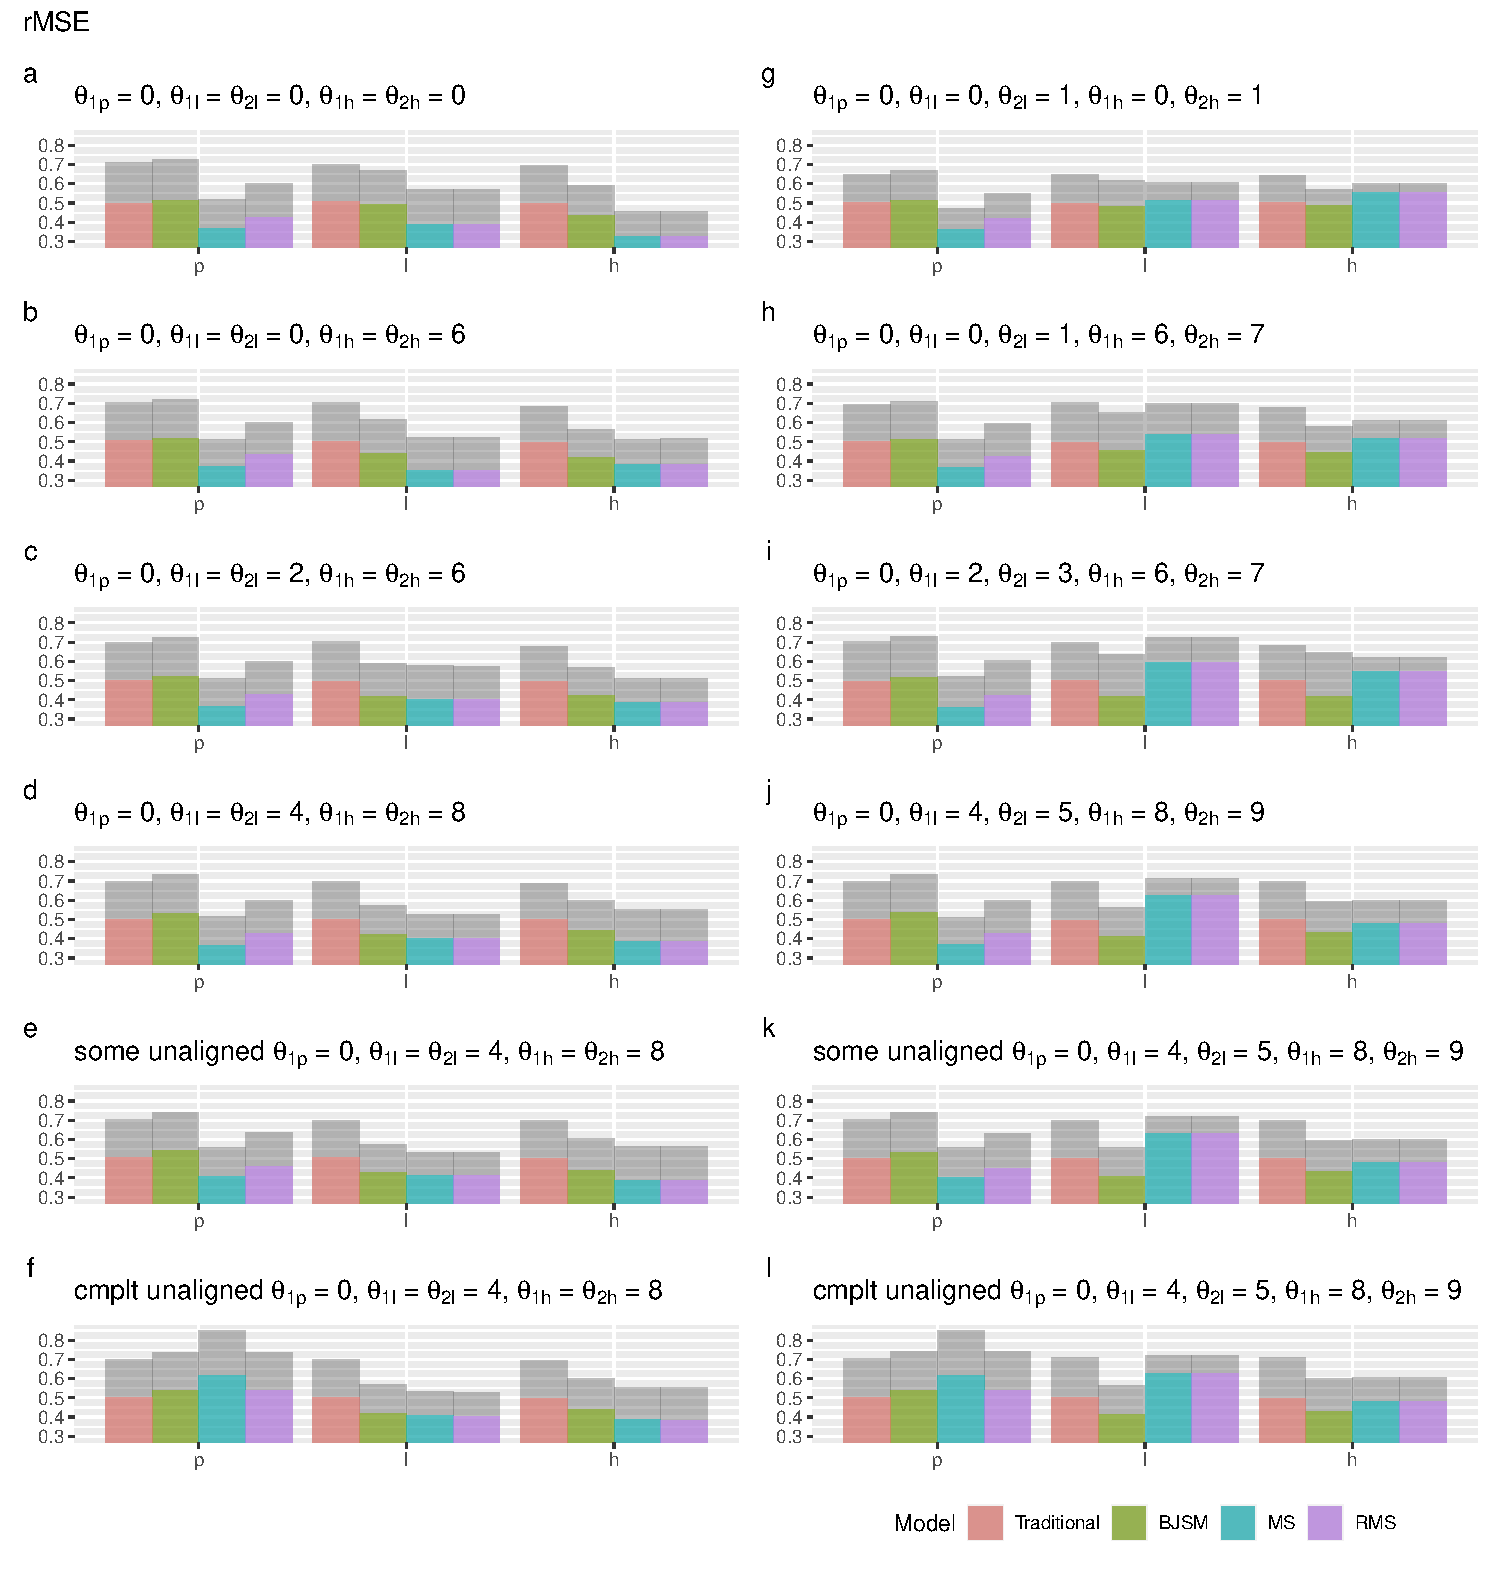
\includegraphics[width=0.95\textwidth]{chapters/figures/Figure3.pdf}
\caption{Simulated root-mean-square error (rMSE) for the estimators of $\theta_{1k}$ \\ $\theta_{jk}$ is the stage $j$ treatment effect of treatment $k$, where $j = 1,2, k = p, l, h$, p = placebo, l = low dose, and h = high dose. Two hierarchical models: MAC-snSMART (MS) and robust MAC-snSMART (RMS) methods are compared against the traditional method and the Bayesian Joint Stage Model (BJSM). The results of total sample size 50 are shown as the colored bars, while the results of total sample size 25 are shown as the overlaying gray bars. The simulation settings are described on the top of each graph, where $\theta_{jk}$ denotes the true value of the expected treatment effects of treatment $k$ in stage $j$, $j = 1, 2$, $k = p, l, h$, and \emph{some/cmplt unaligned} means some/all of the placebo treatment effects in external control data are inconsistent with the placebo treatment effect in the current trial. This figure appears in color in the electronic version of this article, and color refers to that version.}
\label{fig:rMSE}
\end{figure}


\begin{figure}
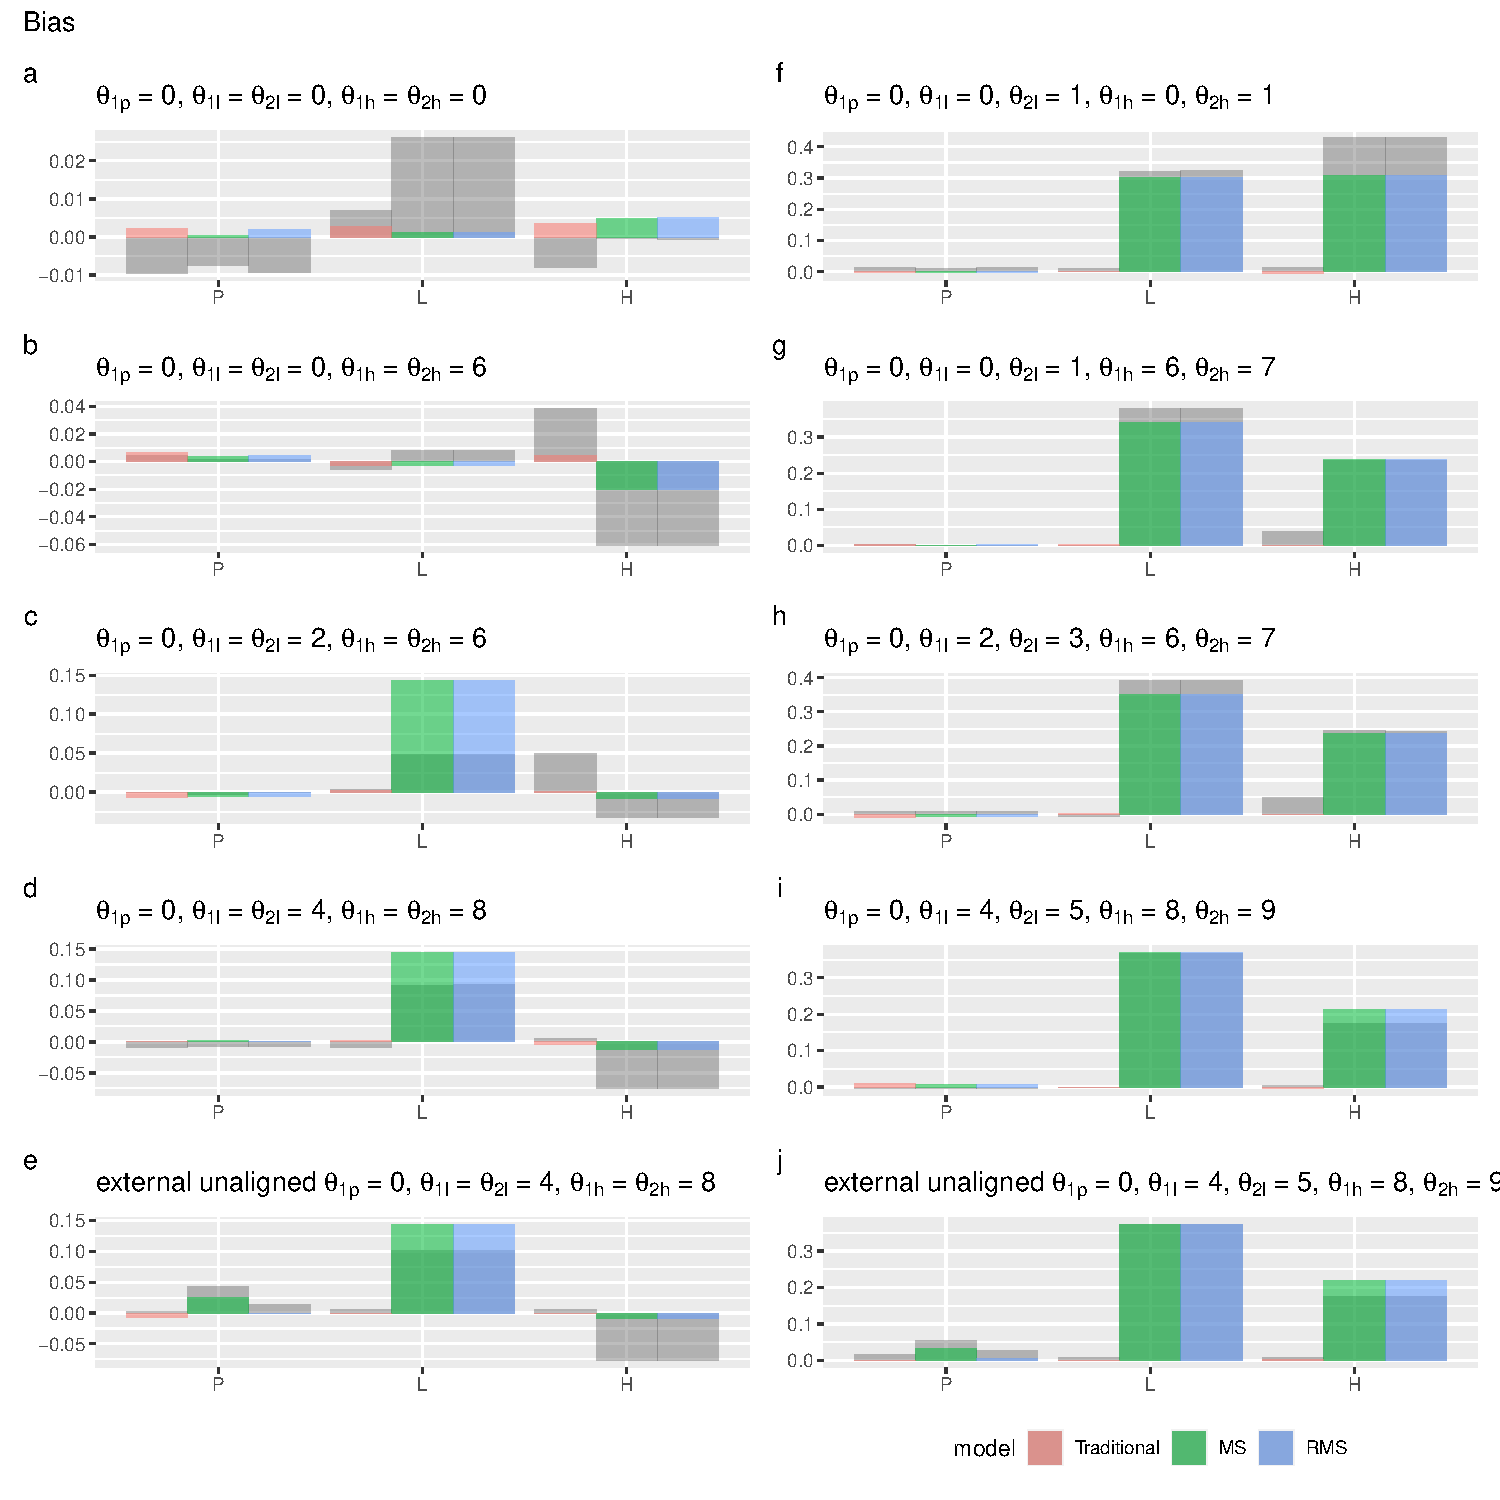
\includegraphics[width=0.95\textwidth]{chapters/figures/Bias1.pdf}
\caption{Simulated bias for the estimators of $\theta_{1k}$. \\ $\theta_{jk}$ is the stage $j$ treatment effect of treatment $k$, where $j = 1,2, k = p, l, h$, p = placebo, l = low dose, and h = high dose. Two hierarchical models: MAC-snSMART (MS) and robust MAC-snSMART (RMS) are compared against the traditional method and the Bayesian Joint Stage Model (BJSM). The results of total sample size 50 are shown as the colored bars, while the results of total sample size 25 are shown as the overlaying grey bars. The simulation settings are described on the top of each graph, where $\theta_{jk}$ denotes the true value of the expected treatment effects of treatment $k$ in stage $j$, $j = 1, 2$, $k = p, l, h$, and \emph{some/cmplt unaligned} means some/all of the placebo treatment effects in external control data are inconsistent with the placebo treatment effect in the current trial. Monte Carlo error (MCE) is smaller than 0.005 for all estimators.}
\label{fig:Bias}
\end{figure}


\begin{figure}
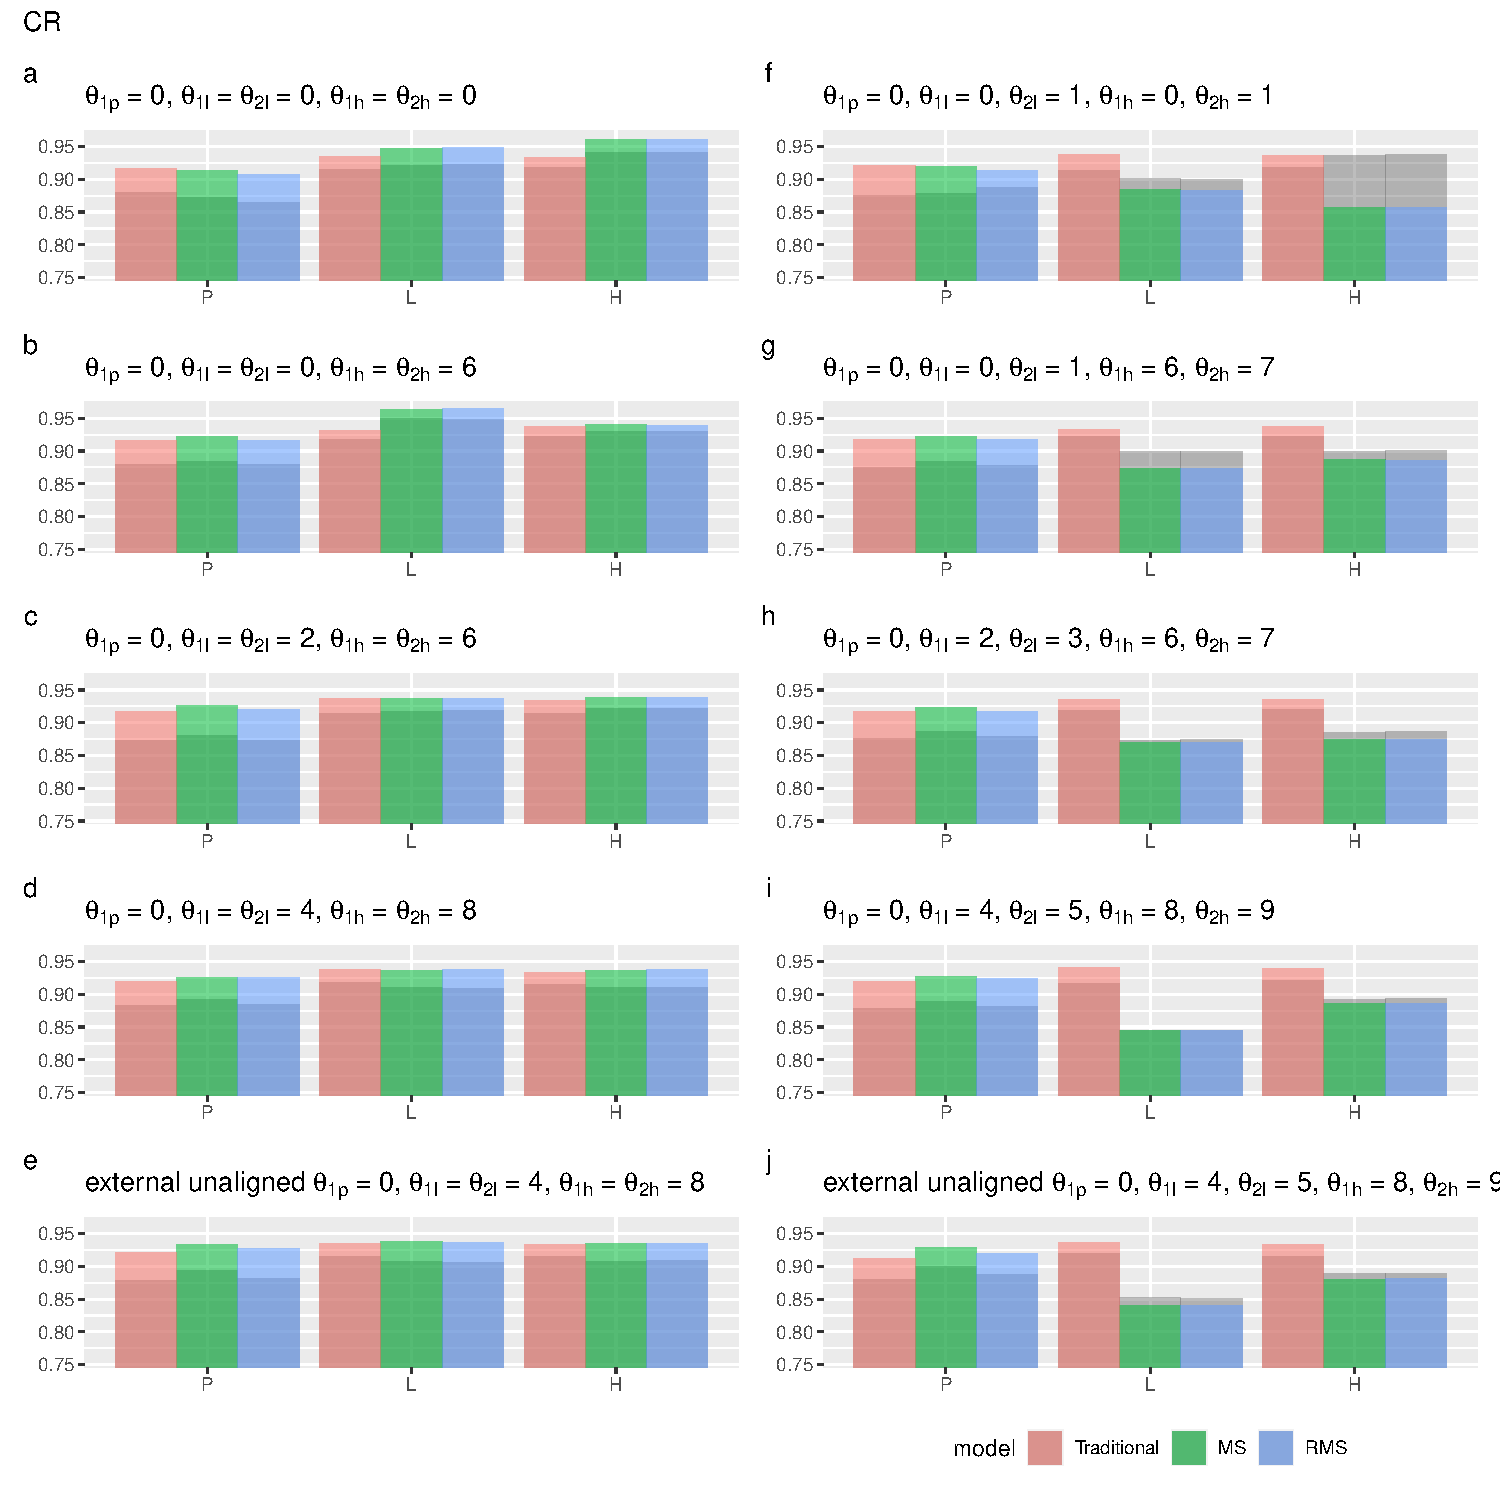
\includegraphics[width=0.95\textwidth]{chapters/figures/CR.pdf}
\caption{Simulated 95\% coverage rate (CR) for the estimators of $\theta_{1k}$.\\ $\theta_{jk}$ is the stage $j$ treatment effect of treatment $k$, where $j = 1,2, k = p, l, h$, p = placebo, l = low dose, and h = high dose. Two hierarchical models: MAC-snSMART (MS) and robust MAC-snSMART (RMS) are compared against the traditional method and the Bayesian Joint Stage Model (BJSM). The results of total sample size 50 are shown as the colored bars, while the results of total sample size 25 are shown as the overlaying grey bars. The simulation settings are described on the top of each graph, where $\theta_{jk}$ denotes the true value of the expected treatment effects of treatment $k$ in stage $j$, $j = 1, 2$, $p, l, h$, and \emph{some/cmplt unaligned} means some/all of the placebo treatment effects in external control data are inconsistent with the placebo treatment effect in the current trial.}
\label{fig:CR}
\end{figure}


\begin{figure}
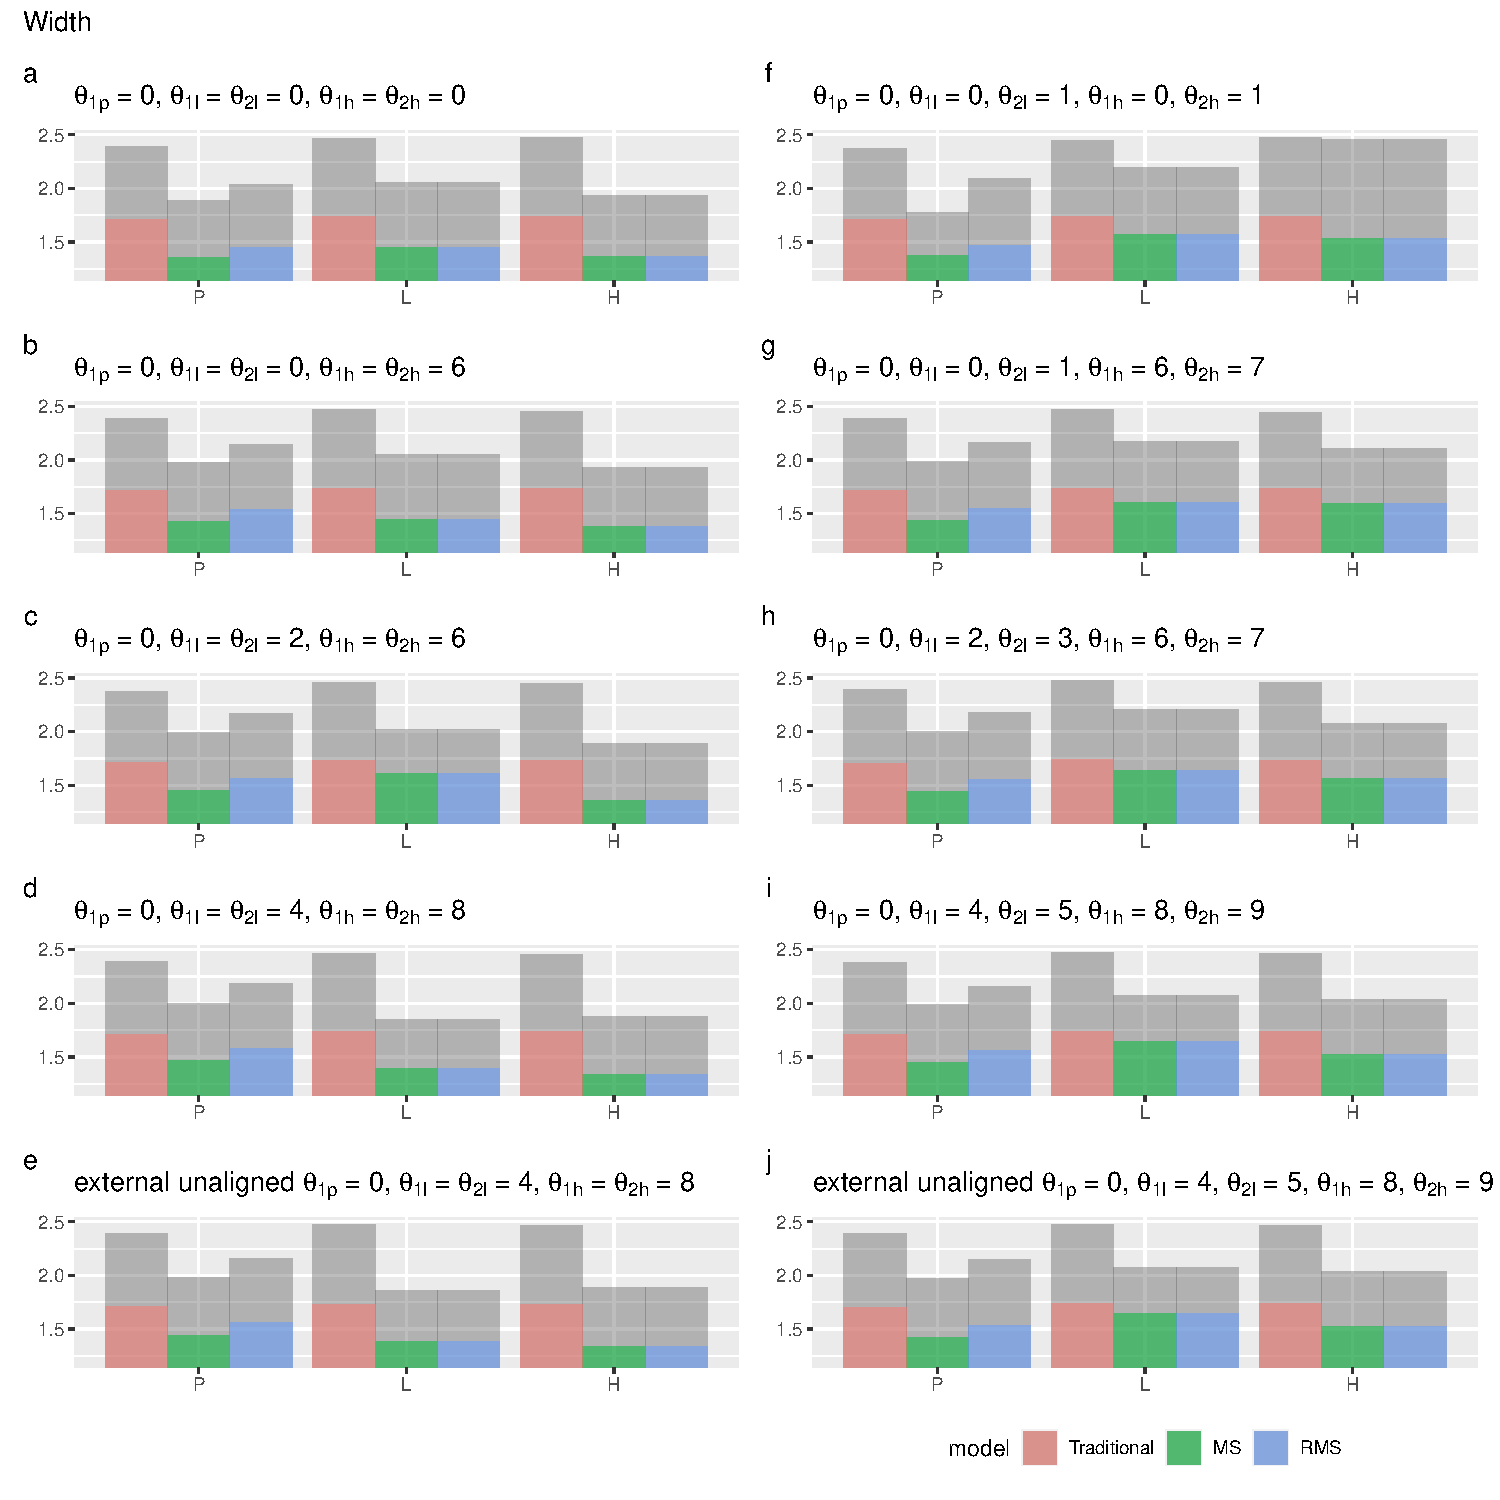
\includegraphics[width=0.95\textwidth]{chapters/figures/Width.pdf}
\caption{Simulated width for the estimators of $\theta_{1k}$. \\ $\theta_{jk}$ is the stage $j$ treatment effect of treatment $k$, where $j = 1,2, k = p, l, h$, p = placebo, l = low dose, and h = high dose. Two hierarchical models: MAC-snSMART (MS) and robust MAC-snSMART (RMS) are compared against the traditional method and the Bayesian Joint Stage Model (BJSM). The results of total sample size 50 are shown as the colored bars, while the results of total sample size 25 are shown as the overlaying grey bars. The simulation settings are described on the top of each graph, where $\theta_{jk}$ denotes the true value of the expected treatment effects of treatment $k$ in stage $j$, $j = 1, 2$, $k = p, l, h$, and \emph{external unaligned} means the placebo treatment effects in external control data are inconsistent with the placebo treatment effect in the current trial. Monte Carlo error (MCE) is smaller than 0.005 for all estimators.}
\label{fig:Width}
\end{figure}

\newpage

\begin{figure}[H]
\centerline{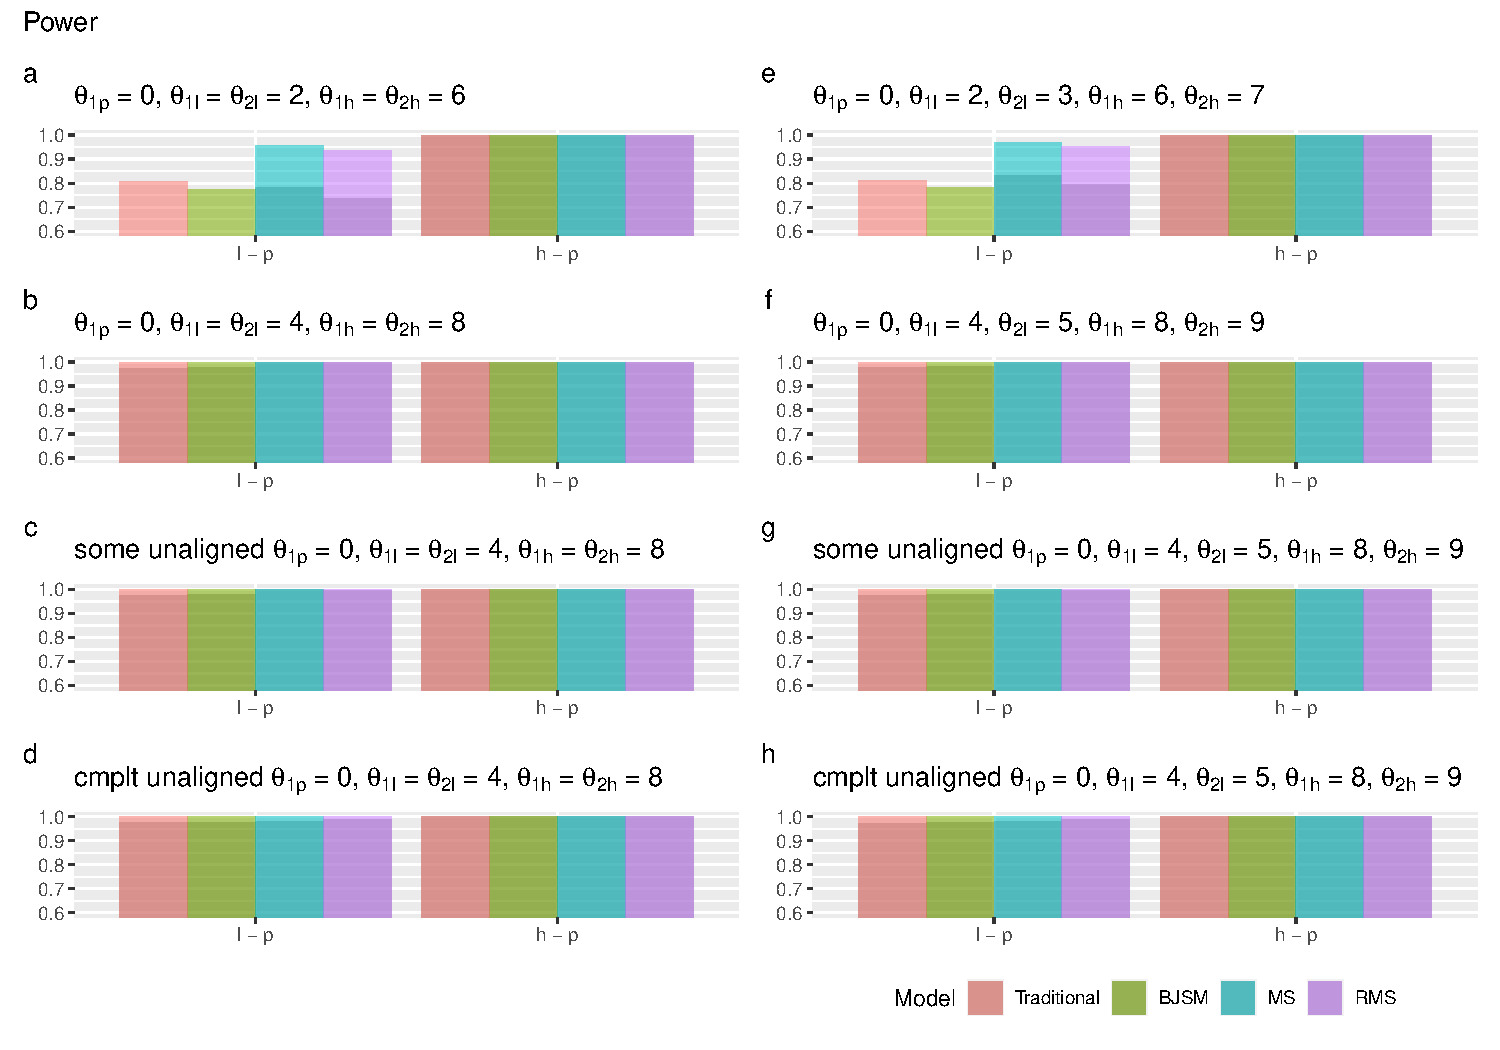
\includegraphics[width=\textwidth]{chapters/figures/CRpower.pdf}}
\caption{Simulated power of the MAC-snSMART methods. \\In this paper, the power is defined as the probability that the credible intervals of $\hat{\theta}_{1l} - \hat{\theta}_{1p}$ and $\hat{\theta}_{1h} - \hat{\theta}_{1p}$ do not include 0 when there are treatment effect difference between low dose and placebo and high dose and placebo. Two hierarchical models: MAC-snSMART (MS) and robust MAC-snSMART (RMS) are compared against the traditional method and the Bayesian Joint Stage Model (BJSM). The results of total sample size 50 are shown as the colored bars, while the results of total sample size 25 are shown as the overlaying grey bars. The simulation settings are described on the top of each graph. $\theta_{jk}$ denotes the true value of the expected treatment effects of treatment $k$ in stage $j$, where $j = 1, 2$, $k = p, l, h$, p = placebo, l = low dose, and h = high dose. \emph{some/cmplt unaligned} means some/all of the placebo treatment effects in external control data are inconsistent with the placebo treatment effect in the current trial.}
\label{fig:Power}
\end{figure}


The right columns of Figure \ref{fig:rMSE}, \ref{fig:Bias}, \ref{fig:CR}, and \ref{fig:Width} present the \ac{rMSE}, average bias,  \ac{CR} , and average \ac{CI} width for estimators of the treatment effects when data are generated violating the exchangeability assumption between stage 1 and 2 (data generating process 2). Due to information borrowing across both stages, the MAC-snSMART leads to larger positive average biases and subsequently lower coverage rates and higher \ac{rMSE} values compared to the traditional method. The decrease in  \ac{CR}  can be mitigated by setting a larger standard deviation for the half-normal prior of $\tau_k$ or incorporating the robustification component (Section \ref{sec:robust}) into the distribution of $\theta_{2k'}$ in Formula \ref{eq:joint}. The \ac{BJSM} is less susceptible to this issue since a ``shift" parameter $\alpha$ is incorporated in the model \citep{fang2023comparing}. Under this data generation setting, the traditional method provides the best placebo treatment effect estimators among the presented methods, and the \ac{BJSM} provides the best low and high dose treatment effect estimators. Conclusions were consistent for sample size 25 under both data generation processes and all scenarios.

Table \ref{tab:TypeI} and Figure \ref{fig:Power} present the type I error and power of each model. The MAC-snSMART methods have smaller type I errors than the traditional method when its assumption of full exchangeability between stages is upheld, and the type I error is still reasonable (below 0.1) when this assumption is violated. The \ac{BJSM} has the smallest type I error when the exchangeability assumption between two stages is violated. When the treatment effect is clinically meaningful (i.e., $\geqslant 4$), all methods have power close to 1 under all scenarios and sample sizes. The MAC-snSMART methods have a significant increase in power compared to the traditional method and the \ac{BJSM} when the treatment effect is equal to 2. The power gain is even greater for a smaller sample size ($n=25$). Overall, the robust MAC-snSMART is the best-performing model when exchangeability of stage-wise treatment effects is upheld.

\section{Re-analysis of SPITFIRE trial} \label{s:example}

To illustrate the practical utility of the proposed \ac{snSMART} design and MAC-snSMART methods, we conducted a reanalysis of the SPITFIRE study. Given that the trial stopped for futility after stage 1, we only have summary-level \ac{NSAA} total scores and \ac{6MWD} at baseline and week 48 (details in Table \ref{tab:study_measure}). To create a data set that matches our proposed trial design, we simulated stage 1 patient-level data by randomly drawing from normal distributions based on the SPITFIRE data. \ac{NSAA} outcome data for placebo ($n=30$), low dose ($n=29$) and high dose ($n=33$) were generated using  $N(-2.99, 0.65^2 \times \sqrt{30})$, $N(-3.44, 0.67^2 \times \sqrt{29})$, and  $N(-2.41, 0.64^2 \times \sqrt{33})$, respectively. As per study protocol, we set a change of $\geqslant -3.1$ points from baseline as the threshold for a clinically meaningful treatment effect \citep{muntoni2018minimal} and to categorize stage 1 responders and nonresponders. Stage 2 patient-level treatment outcomes were again randomly generated using formula \ref{eq:joint} with $s_{kk'}$ randomly chosen between -1 and 1, and low and high dose outcomes drawn from $N(-3.44, 0.67^2\sqrt{n_{2l}})$ and $N(-2.41, 0.64^2\sqrt{n_{2h}})$, respectively. Our proposed \ac{snSMART} design and randomly generated stage 1 outcomes dictated $n_{2l}$ and $n_{2h}$. We followed the same procedure to simulate stage 1 and stage 2 \ac{6MWD} data.


\begin{table}
\caption{\label{tab:study_measure}The SPITFIRE trial study measures. Summary
statistics are reported as mean (SD) for NSAA and 6MWD.}
\vspace{-2.5mm}
\begin{center}
\begin{tabular}{p{4.8cm}p{3cm}p{2.9cm}p{3cm}}
\hline
\centering  & \centering Placebo & \centering RO7239361 Low Dose & \centering RO7239361 High Dose \tabularnewline
\hline
\textit{Baseline} &&&\\
\raggedleft Sample Size & \centering 56 & \centering 55 & \centering 55 \tabularnewline 
\raggedleft NSAA & \centering 23.1  (6.4) & \centering 24.5  (5.5) & \centering 22.7  (6.7) \tabularnewline
\raggedleft 6MWD & \centering 388.33 (69.59) & \centering 399.73 (68.35) & \centering 370.73 (93.35) \tabularnewline
\hline
\textit{Week 48} &&& \tabularnewline
\raggedleft Sample Size - NSAA & \centering 30 & \centering 29 & \centering 33 \tabularnewline 
\raggedleft Changes in NSAA & \centering -2.99  (0.65) & \centering -3.44  (0.67) & \centering -2.41  (0.64) \tabularnewline
\raggedleft Sample Size - 6MWD & \centering 29 & \centering 25 & \centering 31 \tabularnewline 
\raggedleft Changes in 6MWD & \centering -41.3 (8.7) & \centering -39.6 (9.0) & \centering -30.0 (8.7) \tabularnewline
\hline
\end{tabular}
\end{center}
\end{table}

We used \ac{CINRG} \ac{DNHS} data as the source of external control in this re-analysis. Data from \ac{DNHS} participants who met the SPITFIRE trial eligibility criteria and had \ac{NSAA} total score or \ac{6MWD} records were used for the external control group. Our model assumption of exchangeability between external and current trial controls seems valid due to careful selection of control data and similarity of demographics and disease severity in patients. Since the participant visit schedule of \ac{DNHS} was different from the SPITFIRE trial, for each participant, we picked the test record with ``days from baseline'' closest to 336 ($48 \times 7$) as their ``Week 48'' record. Alternatively, we could impute ``Week 48" observations, a method that will be described in Chapter \ref{chpt:longitudinal}. In the end, for \ac{NSAA} total score, data from 25 participants were used for the external control data with a mean \ac{NSAA} total score change from baseline being -1.04 and its standard deviation being 0.77. The same data were used for \ac{6MWD} with a mean \ac{6MWD} change from baseline being -22.36 and its standard deviation being 27.98.

Considering the wide variation in outcomes, 30,000 realizations were simulated for both \ac{6MWD} and \ac{NSAA} total score to assess model performance. When implementing the robust MAC-snSMART method, we carefully followed the prior specification rules outlined in Section \ref{sec:priors}. For example, based on the SPITFIRE stage 1 \ac{NSAA} total scores, most of the observed biases $b_{ll}, b_{lh}$ and $b_h$ should range between 0 and 7. Therefore, we used a conservative uniform distribution $Unif(0, 15)$ as the priors for $B_{ll}, B_{lh}$, and $B_h$ to cover the range. The details of all other prior specifications can be found in the R code provided. 

We fitted the traditional analytic method, \ac{BJSM}, and robust MAC-snSMART method, with results shown in Table \ref{tab:comp}. Notice that the estimators obtained from the robust MAC-snSMART method and \ac{BJSM} are consistent with each other and have significantly smaller \ac{CI} widths than the traditional method because of the efficient use of data across both stages. Thus, even though the \ac{BJSM} and the robust MAC-snSMART reached the same conclusion as the SPITFIRE trial, i.e., failing to reject the null hypothesis, more precise treatment effects estimations were provided by these two methods.  

\begin{table} 
\caption{\label{tab:comp} Example data analysis result comparison. Note: $\widehat{\theta}_{1k}$ is the estimated stage 1 treatment effect or change from baseline to 48 weeks in the NSAA or 6MWD for treatment $k$, where $k = p,l,h$, $p = $ placebo, $l = $ low dose, and $h = $ high dose. Four analytic methods: original SPITFIRE trial results, traditional analytic method, robust MAC-snSMART (RMS), and  Bayesian joint stage modeling (BJSM) are compared. ``NSAA" stands for ``North Star Ambulatory Assessment total score", and ``6MWD" stands for ``6-minute walk distance". The 95\% confidence or credible intervals of the estimates are shown in the parenthesis.}
\centering
%\begin{tabular}{p{2.6cm}p{3.3cm}p{3.3cm}p{3.3cm}p{3.3cm}}
\begin{tabular}{ccccc}
\hline
Estimator &  Original Result &  Traditional &  RMS  & BJSM \tabularnewline
\hline
\multicolumn{1}{l}{\textit{NSAA}} &&&&\\
\multicolumn{1}{r}{$\widehat{\theta}_{1p}$} &  -2.99 (-4.26, -1.71) &  -2.98 (-4.24, -1.73) &  -2.89 (-3.68, -2.10) &  -2.91 (-4.01, -1.82)  \tabularnewline 

\multicolumn{1}{r}{$\widehat{\theta}_{1l}$}  &  -3.44 (-4.75, -2.13) &  -3.44 (-4.74, -2.14) &  -3.40 (-4.49, -2.31) &  -3.38 (-4.34, -2.41)  \tabularnewline

\multicolumn{1}{r}{$\widehat{\theta}_{1h}$} &  -2.41 (-3.66, -1.16) &  -2.41 (-3.65, -1.17)  &  -2.49 (-3.56, -1.42) &   -2.42 (-3.35, -1.48) \tabularnewline

\multicolumn{1}{r}{$\widehat{\theta}_{1l} - \widehat{\theta}_{1p}$} &  -0.45 (-2.17, 1.27) &  -0.46 (-2.27, 1.36)  &  -0.52 (-1.88, 0.83) &  -0.46 (-1.91, 0.98)  \tabularnewline
\multicolumn{1}{r}{$\widehat{\theta}_{1h} - \widehat{\theta}_{1p}$} &  	0.58 (-1.10, 2.26) &  0.58 (-1.20, 2.35)  &  0.40 (-0.94, 1.74) &  0.50 (-0.93, 1.92)\tabularnewline
\hline
\multicolumn{1}{l}{\textit{6MWD}} &&&&\\
\multicolumn{1}{r}{$\widehat{\theta}_{1p}$} &  -41.3 (-58.4, -24.2) &  -41.3 (-58.2, -24.5)  &  -41.0 (-52.5, -29.3) &  -41.1 (-54.4, -27.8) \tabularnewline 

\multicolumn{1}{r}{$\widehat{\theta}_{1l}$} &  -39.6 (-57.2, -22.0) &  -39.6 (-57.0, -22.2)  &  -39.4 (-53.2, -26.1) &  -39.3 (-51.6, -27.6) \tabularnewline

\multicolumn{1}{r}{$\widehat{\theta}_{1h}$} &  -30.0 (-47.1, -12.9) &  -30.0 (-46.7, -13.0)  &  -30.2 (-42.1, -18.0) &   -29.7 (-40.8, -18.7)\tabularnewline

\multicolumn{1}{r}{$\widehat{\theta}_{1l} - \widehat{\theta}_{1p}$} &  1.7 (-21.1, 24.6) &  1.8 (-22.6, 26.0)  &  1.6 (-15.6, 19.1) &  1.8 (-16.6, 19.5)   \tabularnewline
\multicolumn{1}{r}{$\widehat{\theta}_{1h} - \widehat{\theta}_{1p}$} &  11.3 (-11.0, 33.6) &  11.5 (-12.5, 35.4)  &  10.9 (-6.4, 28.1) &  11.4 (-5.8, 28.6) \tabularnewline
\hline
\end{tabular}
\end{table}

%\section{Practical Implementation}
%\label{s:practical}

\section{Discussion} \label{s:discuss}
%Need something in discussion to bring it back to DMD-- what has been done and why would this be better? This may be more clear when you have example data analysis

In this paper, we were motivated by the current drug development paradigm for \ac{DMD} and other similar rare diseases to present an alternative design and Bayesian methods with efficient use of all available evidence including data from both stages and external control. We have proposed a new \ac{snSMART} design and robust MAC-snSMART method to estimate the treatment effect of placebo, low and high doses with a continuous outcome of interest. The robust MAC-snSMART method provides accurate and robust estimators when the expected treatment effect of the same dose level across stages are similar. Our proposed \ac{snSMART} design and robust MAC-snSMART methods are aligned with the mission of \ac{FDA}'s Complex Innovative Design program \citeyearpar{fdaCID}. We have provided guidelines for prior distributions and alternative models for sensitivity analyses in practical implementation. At the planning stage, it is critical to consider a wide number of scenarios (like those presented in Section \ref{s:simulation}) to understand the impact of model assumptions, prior choice, and sample size for the proposed design and analytic method. This exercise is crucial for sponsors and regulators to understand the practical efficiency and robustness of the model.

The proposed robust MAC-snSMART method assumes treatment effects from stages 1 and 2 are exchangeable, which relies on this assumption of stable disease (and an adequate washout period) to assume stable treatment effects across stages. Diseases like \ac{DMD} used as motivation here, corticobasal degeneration (CBD), and familial Mediterranean fever (FMF), which are slower to progress, are good candidates for the proposed \ac{snSMART} design and analytic methods. If first and second stage treatment effects are not similar or there is not an adequate washout period, a multi-stage design and robust exchangeable model may not be appropriate and lead to biased estimation of treatment effects. At the end of the trial, sensitivity analyses that compare results from a traditional analytic method and the robust MAC-snSMART method can be conducted to assess these assumptions. 

The proposed model is tested with extensive simulation studies across various scenarios. The scenarios include incorporating external control data which are consistent and inconsistent with the current trial placebo arm. Note that, this is not equivalent to a simple pooled analysis of external and concurrent control data as the MAC-snSMART model takes into account between-trial heterogeneity. For example, in the SPITFIRE trial re-analysis, the \ac{ESS} for the robust MAC-snSMART analysis is 12, which is less than the sample size of external placebo data ($n=25$). Thus, more data contributing to the placebo will not always be useful for decreasing the number of patients needed on the placebo arm. It depends on the degree of heterogeneity between different data sources.

While, this manuscript concentrates on enriching the control arm, the MAC framework permits enrichment of treatment arms. However, we believe relevant treatment data are less likely to be available for use in dose-finding studies. An exception may be the use of adult data in pediatric drug development, but there is debate and uncertainty surrounding the validity and reliability of extrapolating safety and efficacy data from adult populations to pediatric populations.

It is possible that even a high dose of the investigative treatment cannot provide a clinically meaningful treatment effect by the end of stage 1. Under this scenario, it is not ethical to continue the trial for those who received high dose in stage 1. Hence, in practice, we recommend a stopping rule such that if less than 30\% of patients respond to high dose in stage 1, stage 2 will not be conducted, and all treatment effects will be calculated based on stage 1 data only. There may be additional trade-offs between efficacy and toxicity which are beyond the scope of this manuscript and the subject of some of our future work.

The SPITFIRE trial and many other \ac{DMD} trials incorporate participant demographic and baseline characteristic covariates into their analysis. In the future, we hope to extend the robust MAC-snSMART method to include patient-level covariates. The use of patient-level covariates is discussed in \cite{kotalik2021dynamic} as a way to assess covariate-adjusted exchangeability. The study uses a linear model and the existing multi-source exchangeability models framework to enable borrowing even when marginal treatment effects are different, but covariate-adjusted exchangeability is maintained. Integrating this feature into the \ac{snSMART} approach would broaden borrowing opportunities. In addition, data in \ac{DMD} trials are usually collected in a longitudinal manner with 3 or more visits. In our study, like in SPITFIRE, we employed the commonly used ``change from baseline" as the primary endpoint, which is in line with regulatory standards. The placebo group in our study allows us to assess the possible ``regression to the mean" effect. Although commonly used, it's worth noting that ``change from baseline" may not always be the most appropriate measure. Our approach remains valid if using the absolute outcome at the end of each stage, and the performance of our method is not affected. If absolute outcomes are used, we can examine the credible intervals in the difference of the differences among the high dose, low dose, and placebo groups. Alternatively, it is important for future work to investigate ways to incorporate longitudinal data into our analytic methods.